\documentclass[11pt,oneside,openany]{book}
\usepackage{zlc_frontend_notes}

\begin{document}
\frontmatter
\zlctitlepage{ZLC 设备与实验手册}{设备配置/加载 / 相机读出原理 / 标定与结果对象 / 实验流程}{devices 层契约、camera capture/readout 教程(sitemap/thresholds/detect)、TrapCalibration、虚拟后端与完整实验循环}{2026-06-05}
\tableofcontents
\cleardoublepage
\mainmatter

\chapter{写给新读者}

\section{为什么单独一本设备与实验手册}
主手册讲系统总览，frontend 手册讲 GUI 与绘图，fpga 手册讲脉冲序列器硬件。但一台真实的中性原子实验还有一整层东西没讲清楚：\tfocus{设备怎么配置和加载、相机怎么采图、原始图像怎么变成"每个格点有没有原子"、一次实验的完整流程长什么样}。这本手册专门补这一层，面向\tfocus{第一次接手这套代码、想跑通一次成像+读出}的人。

\begin{description}
  \item[\pyapi{devices/}] 硬件适配器与设备契约。\filepath{base.py}（设备基类）、\filepath{registry.py}（配置加载）、\filepath{virtual.py}（离线模拟）、\filepath{qcmos.py}（真实相机）、\filepath{sequencer.py}（脉冲序列器客户端）。
  \item[\pyapi{core/}] 纯算法与结果对象。\filepath{calibration.py}（\pyapi{TrapCalibration}）、\filepath{analysis.py}（找格点、阈值、检测）、\filepath{results.py}（结果对象）。
  \item[\pyapi{subsystems/}] 实验级能力束。\pyapi{exp.readout}（读出）、\pyapi{exp.timing}（时序）。
  \item[\pyapi{views/}] 接到 frontend 的绘图适配器（在原始图上叠格点圈）。
\end{description}

\begin{notebox}[一个贯穿全书的不变式]
\pyapi{exp.camera.capture()} 只显示\tfocus{原始}相机图像，永远不画格点圈或阈值叠加。格点圈、占据判定属于\tfocus{读出结果}（\pyapi{sitemap}/\pyapi{detect}），不属于相机设备。如果你在一张 capture 上看到了格点圈，说明把标定状态错放进了相机层。
\end{notebox}

\section{三种后端，同一套 notebook 接口}
\pyapi{na.connect} 返回一个 \pyapi{NeutralAtomSession}，三种典型连法\tfocus{暴露完全相同的接口}，只是底层设备不同：

\begin{figure}[htbp]
  \centering
  \begin{tikzpicture}[font=\footnotesize, node distance=5mm,
      b/.style={draw=StarkGray, rounded corners=2pt, fill=StarkPale, align=center, inner sep=4pt, text width=34mm, minimum height=12mm},
      hw/.style={b, fill=StarkTint}]
    \node[b] (v) {\textbf{virtual}\\VirtualCamera +\\VirtualSequencer +\\VirtualTrapArray\\(完全离线)};
    \node[hw, right=8mm of v] (q) {\textbf{qCMOS + 本地}\\QCMOSCamera +\\RuntimeSequencer\\(本地编译执行)};
    \node[hw, right=8mm of q] (r) {\textbf{qCMOS + 远程 FPGA}\\QCMOSCamera +\\RemoteSequencer\\(RPyC -> FPGA 电脑)};
  \end{tikzpicture}
  \caption{三种后端共享 \pyapi{NeutralAtomSession} 接口。教学/回归用 virtual，真实实验用 qCMOS + 本地或远程序列器。}
  \label{fig:dev-backends}
\end{figure}

\begin{codeblock}[Python]
import Zou_lab_control.neutral_atom as na

# 1) 完全离线：虚拟相机 + 虚拟序列器（教学、写代码、回归测试）
exp = na.connect("virtual")

# 2) 真实硬件：控制电脑连 FPGA 电脑上的 server
exp = na.connect("remote_template",
                 sequencer={"host": "192.168.0.20", "port": 18861},
                 open_devices=True)
\end{codeblock}

session 暴露四个子系统/设备入口：\pyapi{exp.devices}（底层设备集）、\pyapi{exp.camera}（采图）、\pyapi{exp.timing}（脉冲/触发）、\pyapi{exp.readout}（标定与占据检测）。

\chapter{设备配置与加载}

\section{配置就是一个字典}
设备由一份\tfocus{配置}描述，可以是内置名字（\pyapi{"virtual"}）、一个 \filepath{.json} 路径、或一个 Python 字典。结构是\tfocus{每个设备一条 \pyapi{\{type, params\}}}：

\begin{codeblock}[设备配置 JSON]
{
  "trap_array": { "type": "VirtualTrapArray", "params": { "grid_shape": [5, 7] } },
  "camera":     { "type": "VirtualCamera",   "params": { "trap_array": "$device:trap_array" } },
  "sequencer":  { "type": "VirtualSequencer", "params": {} }
}
\end{codeblock}

\begin{description}
  \item[\pyapi{type}] 设备类名（内置短名，或完整 import 路径）。
  \item[\pyapi{params}] 构造参数。\pyapi{"\$device:name"} 表示\tfocus{引用另一台已加载设备}（如相机引用 trap\_array）。加载器按依赖顺序实例化，并检测环。
\end{description}

\section{load\_devices 与 DeviceSet}
\pyapi{na.load_devices(config)}（\filepath{registry.py}）解析配置、按依赖顺序实例化，返回一个 \pyapi{DeviceSet} 容器：

\begin{codeblock}[Python]
devices = na.load_devices("virtual", open_devices=False)
devices.camera        # -> CameraDevice（带类型契约校验）
devices.sequencer     # -> SequencerDevice
devices.trap_array    # -> TrapArrayDevice
devices.snapshot()    # -> {"camera": {...}, "sequencer": {...}, ...} JSON 安全自省
devices.open()        # 按依赖顺序打开（相机最后开），失败时逆序回滚
\end{codeblock}

\pyapi{DeviceSet} 既是属性访问（\pyapi{.camera}）也是字典访问（\pyapi{devices["camera"]}）；\pyapi{.require(name, expected\_type)} 会校验类型契约。

\section{设备注册表}
内置设备类在 \pyapi{DEVICE_CLASSES}（\filepath{registry.py}）：\pyapi{QCMOSCamera}、\pyapi{VirtualCamera}、\pyapi{VirtualTrapArray}、\pyapi{RuntimeSequencer}、\pyapi{RemoteSequencer}、\pyapi{ManualSequencer}、\pyapi{VerilogSequencer}。自定义设备用 \pyapi{na.register_device_class(name, cls)} 注册后即可在配置里按名字引用。

\begin{codeblock}[Python]
na.available_device_configs()   # 列出 configs/ 下可用配置名
na.register_device_class("MyCamera", "mypkg.devices:MyCamera")
\end{codeblock}

\section{设备契约（四种类型）}
所有设备继承 \pyapi{BaseDevice}（\pyapi{open/close/stop/snapshot}）。三个\tfocus{类型化}子类是强约束（用 \pyapi{isinstance} 校验，不是鸭子类型）：

\begin{description}
  \item[\pyapi{CameraDevice}] \pyapi{exposure} 属性、\pyapi{configure(exposure=...)}、\pyapi{acquire(frames, sequence, sequencer) -> list[np.ndarray]}、便捷的 \pyapi{capture(...) -> CaptureResult}、\pyapi{bind_experiment(session)}。
  \item[\pyapi{SequencerDevice}] \pyapi{channels}、\pyapi{clock_hz}、\pyapi{prepare(sequence)}、\pyapi{fire(sequence=None)}；可选 \pyapi{wait_done(timeout)}、\pyapi{abort()}、\pyapi{set_safe_state()}。
  \item[\pyapi{TrapArrayDevice}] \pyapi{n_sites}。刻意精简：它\tfocus{不}暴露相机像素坐标的格点中心（那是标定的产物）。\pyapi{VirtualTrapArray} 额外有 \pyapi{grid_shape}/\pyapi{occupancy}/\pyapi{render_image()}/\pyapi{reload()}。
\end{description}

\chapter{相机采集原理}

\section{capture 返回什么}
\pyapi{exp.camera.capture(frames=1, exposure=None, display=True)} 抓若干帧，返回一个 \pyapi{CaptureResult}：

\begin{codeblock}[Python]
res = exp.camera.capture(frames=1, display=True)
res.images     # list[np.ndarray]，原始 uint16 帧
res.image      # 便捷取最后一帧
res.plot       # frontend 绘图对象（只画原始像素，无任何叠加）
\end{codeblock}

\pyapi{capture()} 内部调 \pyapi{acquire(frames, sequence, sequencer)}：若提供了序列器，会先把成像序列扩展到所需帧数，\pyapi{prepare()} 上传、\pyapi{fire()} 启动，相机用外触发采集，之后 \pyapi{wait_done()}。这是\tfocus{相机和序列器协同}的唯一入口。

\begin{notebox}[曝光时间的真相来源]
曝光既能在相机上设（\pyapi{camera.configure(exposure=...)}），也写在脉冲序列里（probe 脉冲宽度）。约定：\tfocus{序列里的曝光是真相来源}；相机应当从序列取曝光，而不是反过来。改曝光时优先改成像序列（\pyapi{exp.timing.configure_imaging(exposure=...)}）。
\end{notebox}

\section{虚拟相机怎么造图}
\pyapi{VirtualCamera}（\filepath{virtual.py}）用 \pyapi{trap_array.render_image()} 合成图：每个被占据的格点画一个高斯 PSF，叠泊松噪声，按曝光与原子寿命采样。它让你\tfocus{不接硬件也能跑通整条读出链路}做开发和回归。

\begin{notebox}[虚拟 vs 真实的一个差异]
虚拟相机在采\pyapi{名为 "sitemap" 的序列}时会强制"所有格点都加载"（方便标定）。真实硬件没有这个隐藏行为——做 sitemap 时你必须自己保证原子都加载好。把这条记在心里，别被虚拟后端的"理想 sitemap"误导。
\end{notebox}

\chapter{相机读出教程：从原始图到占据}

读出分三步，每步产出一个\tfocus{标定}并存进 session：\textbf{找格点（sitemap）} -> \textbf{学阈值（thresholds）} -> \textbf{单张检测（detect）}。

\begin{figure}[htbp]
  \centering
  \begin{tikzpicture}[font=\scriptsize, node distance=6mm,
      s/.style={draw=StarkTeal, rounded corners=2pt, fill=StarkCodeBack, align=center, inner sep=4pt, text width=33mm, minimum height=15mm},
      arr/.style={-{Latex[length=2mm]}, StarkBlue, thick}]
    \node[s] (a) {\textbf{sitemap}\\平均多帧 -> 找峰\\-> 格点中心(像素)\\TrapCalibration.centers};
    \node[s, right=9mm of a] (b) {\textbf{thresholds}\\每格点 ROI 计数\\Otsu 分亮/暗\\TrapCalibration.thresholds};
    \node[s, right=9mm of b] (c) {\textbf{detect}\\单张图每格点\\counts > threshold\\-> occupied 布尔};
    \draw[arr] (a) -- (b); \draw[arr] (b) -- (c);
  \end{tikzpicture}
  \caption{读出三步：sitemap 定位、thresholds 学边界、detect 判占据。前两步是标定（每次实验做一次），detect 是逐张测量。}
  \label{fig:readout-flow}
\end{figure}

\section{第一步：sitemap（定位格点中心）}
\begin{codeblock}[Python]
sm = exp.readout.sitemap(frames=20, grid_shape=(5, 7), ordering="row-major",
                         roi_radius=1, reducer="mean", display=True)
sm.calibration.centers   # (35, 2) 每个格点的 (x, y) 像素坐标
sm.average_image         # 多帧平均图
sm.plot                  # 平均图 + 格点圈叠加
\end{codeblock}

\textbf{原理}（\filepath{analysis.py} 的 \pyapi{find_site_centers}）：平均所有帧 -> 高斯平滑去噪 -> 局部极大值找峰 -> 按相对阈值筛掉背景 -> 按网格顺序（row-major / serpentine / ...）排序，得到稳定的 \pyapi{(N\_sites, 2)} 像素中心。\tfocus{sitemap 假设所有阱都被占据}，它是标定不是测量。

\section{第二步：thresholds（学亮/暗边界）}
\begin{codeblock}[Python]
exp.readout.sitemap(frames=6, display=False)        # 必须先有 sitemap
th = exp.readout.thresholds(frames=100, site=0, display=True)
th.calibration.thresholds   # (35,) 每个格点一个 Otsu 阈值
th.counts                   # (100, 35) 每帧每格点的 ROI 计数
th.fidelity                 # 所显示格点的判别保真度估计
\end{codeblock}

\textbf{原理}：对每帧每格点取 \pyapi{roi_counts}（中心周围 \pyapi{NxN} 像素盒，按 \pyapi{reducer} 归约成一个标量计数）。把 100 次的计数直方图化，用 \pyapi{otsu_threshold} 找\tfocus{最大化类间方差}的阈值，把"暗"（~0–5 计数，背景+读出噪声）和"亮"（~50–200 计数，原子荧光）分开。保真度 \pyapi{estimate_threshold_fidelity} 用两个正态拟合亮/暗分布、算重叠积分得到。

\begin{figure}[h]
\centering
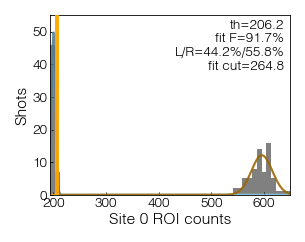
\includegraphics[width=0.6\linewidth]{assets/device_threshold_hist.png}
\caption{虚拟后端\tfocus{实跑}的 thresholds 标定直方图（Site 0，120 帧）：左峰为\tfocus{暗}态（背景+读出噪声），右峰为\tfocus{亮}态（原子荧光），并叠加亮/暗高斯拟合；图中标注了 Otsu 阈值、拟合保真度与亮/暗占比。\pyapi{detect} 时把单张图每格点的 ROI 计数与该阈值逐位比较，得占据布尔；两峰分得越开、保真度越接近 1。本图由读出标定 \pyapi{thresholds} 的 \pyapi{plot_site} 直接产出，而非示意图。}
\end{figure}

\begin{notebox}[reducer 必须前后一致]
阈值是\tfocus{针对某个 reducer}（mean/sum/...）学出来的。检测时若换了 reducer，阈值就对不上。保持整次实验同一个 reducer（存在 \pyapi{TrapCalibration.reducer} 里）。
\end{notebox}

\section{第三步：detect（单张图判占据）}
\begin{codeblock}[Python]
det = exp.readout.detect(display=True, what="occupancy")
det.detection.occupied          # (35,) 布尔，每格点有没有原子
det.detection.occupied_indices  # [被占据格点的下标]
det.detection.counts            # (35,) 该张图每格点的计数
det.plot                        # 原始图 + 被占据格点亮圈
\end{codeblock}

\textbf{原理}（\pyapi{detect_atoms}）：取单张图每格点的 ROI 计数，逐元素 \pyapi{counts > thresholds} 得布尔占据数组。这是\tfocus{基于阈值的二元分类}，每张图独立判断，没有多帧贝叶斯/卡尔曼。

\section{检测时间扫描（保真度 vs 曝光）}
\begin{codeblock}[Python]
scan = exp.readout.detection_time(times=[5e-6, 2e-5, 1e-4], shots=60,
                                  live=True, display=True)
scan.times          # (3,) 各检测曝光时间（秒）
scan.fidelities     # 每个时间点的判别保真度
scan.stop()         # 提前停（live 模式）
\end{codeblock}

先在长曝光下采一组\tfocus{参考}图建参考阈值，再对每个检测时间采 \pyapi{shots} 张、算 Otsu 阈值与保真度。用它选一个"保真度已到平台"的成像时间。

\chapter{标定与结果对象}

\section{TrapCalibration}
读出三步的产物都封装在 \pyapi{TrapCalibration}（\filepath{core/calibration.py}）：

\begin{description}
  \item[\pyapi{centers}] \pyapi{(N, 2)} 格点中心像素坐标。
  \item[\pyapi{thresholds}] \pyapi{(N,)} 每格点阈值（或标量）。
  \item[\pyapi{grid_shape}] 阵列形状 \pyapi{(ny, nx)}。
  \item[\pyapi{roi_radius}] ROI 半径（计数用的像素盒大小）。
  \item[\pyapi{reducer}] 归约方式 \pyapi{"mean"/"sum"/"median"/"max"}。
  \item[\pyapi{metadata}] 任意标志，如 \pyapi{\{"thresholds_calibrated": True\}}。
\end{description}

\begin{codeblock}[Python]
path = exp.readout.save("calib.json")     # 存 .json（可读）或 .npz（紧凑）
exp.readout.load(path)                     # 载回，设到 exp 当前标定
exp.readout.current                        # 当前 TrapCalibration | None
exp.readout.clear()                        # 丢弃当前标定
cal = na.TrapCalibration.load("calib.json")
cal.detect(image)                          # 直接用标定检测一张图
\end{codeblock}

\section{结果对象与 history}
每个读出/采集操作返回一个\tfocus{notebook 友好}的结果对象（\pyapi{CaptureResult}/\pyapi{SitemapResult}/\pyapi{ThresholdResult}/\pyapi{DetectionResult}/\pyapi{DetectionTimeScanResult}），都带一个 \pyapi{.plot}，并自动追加进 \pyapi{exp.history}，方便事后复盘与导出。

\begin{notebox}[叠加是非破坏性的]
格点圈是画在 matplotlib 坐标轴上的，\tfocus{从不修改原始图像数组}。sitemap/detect 的 \pyapi{.plot} 有圈，\pyapi{capture()} 的没有——同一张原始图，圈只是视觉层。
\end{notebox}

\chapter{一次实验完整走一遍}

\section{典型 notebook 循环}
\begin{codeblock}[Python]
import Zou_lab_control.neutral_atom as na

# 0) 连接（离线先用 virtual 跑通）
exp = na.connect("virtual")

# 1) 配成像时序（曝光是真相来源）
exp.timing.configure_imaging(exposure=2e-3, load=True)
exp.timing.preflight().raise_if_failed()        # 跑前自检：对齐/约束

# 2) 读出标定：定位 -> 学阈值
exp.readout.sitemap(frames=20, grid_shape=(5, 7), display=True)
exp.readout.thresholds(frames=100, display=True)
exp.readout.save("calib.json")

# 3) 单张检测
det = exp.readout.detect(display=True)
print("loaded:", det.detection.occupied_indices)

# 4) 扫描测量（live 画图）
scan = exp.readout.detection_time(times=[5e-6, 2e-5, 1e-4], shots=60, live=True)
\end{codeblock}

\section{脉冲、扫描与读出怎么衔接}
\pyapi{exp.timing} 拥有当前 \pyapi{PulseSequence}，并能 \pyapi{bind_pulse(pulse)} 把一个 GUI 脉冲或 \pyapi{PulseTableState} 绑到序列器做扫描（详见主手册的 N-slot 扫描模型与 fpga 手册）。一次"扫描 + 采集"的闭环：绑定脉冲与扫描表 -> 相机 arm -> 序列器 \pyapi{prepare/fire} 逐扫描点无缝迭代、每点触发一次相机 -> 逐张 \pyapi{detect} -> 把每点占据/计数汇成 1D/2D 结果画出来。

\begin{notebox}[有限帧 vs 自由循环]
真实相机采有限帧时，应让 readout/camera helper 先 arm 相机，再生成\tfocus{刚好需要帧数}的有限触发序列；不要让 qCMOS 去等一个没有帧数边界的 \pyapi{repeat_forever} 自由循环脉冲（那适合示波器找线，不适合定量采集）。
\end{notebox}

\chapter{离线虚拟后端}
\pyapi{na.connect("virtual")} 给你一套完全离线的 \pyapi{VirtualCamera + VirtualSequencer + VirtualTrapArray}。它对写实验逻辑、回归测试、教学非常有用：整条 sitemap/thresholds/detect/scan 链路都能跑，不接任何硬件。\pyapi{VirtualTrapArray} 可设 \pyapi{occupancy}、\pyapi{reload()} 重新随机装载、\pyapi{render_image()} 出图。本仓库的大量测试就跑在虚拟后端上。

\chapter{设备配置与加载（深入）}

本章是给"从零开始"理解本系统设备层的人写的一份参考手册。它回答四个核心问题：一份\tfocus{设备配置}长什么样、\pyapi{load_devices} 与 \pyapi{DeviceSet} 如何把配置变成可用的设备对象、所有设备共同遵守的\tfocus{契约}（contract）是什么、以及在五个时序器（sequencer）类之间如何取舍。每一节都尽量给出可直接运行的代码片段，并标注常见错误。

\section{设备层的文件地图}

设备层全部位于 \filepath{Zou_lab_control/neutral_atom/devices/} 目录下。先建立一张文件与职责的对照表，后面各节会反复引用。

\begin{description}
\item[\filepath{devices/base.py}] 定义抽象基类：\pyapi{BaseDevice} 是所有设备的根，三个领域基类 \pyapi{CameraDevice}、\pyapi{SequencerDevice}、\pyapi{TrapArrayDevice} 在其上扩展各自的领域方法。它们规定了"一个设备必须提供哪些方法"，即设备契约。
\item[\filepath{devices/registry.py}] 注册表与加载器。包含 \pyapi{load_devices}、\pyapi{DeviceSet}、\pyapi{DEVICE_CLASSES}、\pyapi{register_device_class}、\pyapi{available_device_configs}、\pyapi{read_config}。这是你与设备层打交道的主入口。
\item[\filepath{devices/virtual.py}] 离线模拟实现：\pyapi{VirtualCamera}、\pyapi{VirtualTrapArray}、\pyapi{VirtualSequencer}。没有任何真实硬件时用它们跑通整条流程。
\item[\filepath{devices/qcmos.py}] \pyapi{QCMOSCamera}，真实的 qCMOS 相机驱动封装。
\item[\filepath{devices/sequencer.py}] 几个真实/半真实时序器实现（\pyapi{RuntimeSequencer}、\pyapi{RemoteSequencer}、\pyapi{ManualSequencer}、\pyapi{VerilogSequencer}）的设备层包装。
\end{description}

\begin{notebox}[心智模型]
配置（一段 JSON 或 dict）是\tfocus{描述}，\pyapi{load_devices} 是\tfocus{工厂}，\pyapi{DeviceSet} 是\tfocus{已经造好、可以打开使用的一组设备}。三者层层递进：先写描述，再实例化，最后打开。
\end{notebox}

\section{一份配置长什么样}

配置可以是三种形态之一，\pyapi{read_config} 与 \pyapi{load_devices} 都接受它们：

\begin{enumerate}
\item 字符串 \pyapi{"virtual"}：一个内置快捷方式，等价于加载内置的全虚拟配置（虚拟相机 + 虚拟时序器 + 虚拟阱阵列），用于无硬件冒烟测试。
\item 一个 \filepath{.json} 文件路径：磁盘上的配置文件。
\item 一个 Python \pyapi{dict}：在代码里直接构造的配置，跳过磁盘。
\end{enumerate}

无论哪种形态，最终的数据结构是统一的：顶层是一个字典，键是\tfocus{设备名}（device\_name，你自己取的逻辑名字，例如 \pyapi{"cam"}、\pyapi{"seq"}），值是一个描述该设备的小字典，含两个字段：

\begin{description}
\item[\pyapi{"type"}] 设备类的\tfocus{短名}（ClassName），例如 \pyapi{"VirtualCamera"}。短名通过 \pyapi{DEVICE_CLASSES} 映射到真正的类。
\item[\pyapi{"params"}] 传给该类构造函数的参数字典。可以为空 \pyapi{\{\}}。
\end{description}

\subsection{最小 JSON 示例}

下面是一份完整、自洽的虚拟配置。把它存成 \filepath{my_virtual.json} 即可被 \pyapi{load_devices} 加载：

\begin{codeblock}[Python]
{
  "trap": {
    "type": "VirtualTrapArray",
    "params": { "n_sites": 16 }
  },
  "seq": {
    "type": "VirtualSequencer",
    "params": { "channels": 62, "clock_hz": 50000000 }
  },
  "cam": {
    "type": "VirtualCamera",
    "params": { "exposure": 0.01 }
  }
}
\end{codeblock}

注意三个键 \pyapi{trap}/\pyapi{seq}/\pyapi{cam} 是\tfocus{你取的名字}，不是固定关键字；\pyapi{DeviceSet} 会根据每个设备的\tfocus{类型}（是相机/时序器/阱阵列）自动把它归类到 \pyapi{.camera}/\pyapi{.sequencer}/\pyapi{.trap\_array}，而不是看名字。

\subsection{等价的 Python dict 示例}

完全相同的配置在代码里这样写，可直接喂给 \pyapi{load_devices}：

\begin{codeblock}[Python]
config = {
    "trap": {"type": "VirtualTrapArray", "params": {"n_sites": 16}},
    "seq":  {"type": "VirtualSequencer", "params": {"channels": 62,
                                                    "clock_hz": 50_000_000}},
    "cam":  {"type": "VirtualCamera",    "params": {"exposure": 0.01}},
}

from Zou_lab_control.neutral_atom.devices.registry import load_devices
devices = load_devices(config)   # 返回一个 DeviceSet
\end{codeblock}

\subsection{设备之间的依赖：\pyapi{\$device:name}}

\pyapi{params} 里的某个值如果写成字符串 \pyapi{"\$device:name"}，表示"把另一个已经构造好的设备对象注入到这里"。这是设备之间互相引用的唯一机制。典型用途是让相机持有时序器的引用，或让某个组合设备依赖底层设备。

\begin{codeblock}[Python]
config = {
    "seq": {"type": "VirtualSequencer", "params": {"channels": 62}},
    "cam": {
        "type": "VirtualCamera",
        "params": {
            "exposure": 0.01,
            "sequencer": "$device:seq"   # 注入上面那个 seq 设备对象
        }
    },
}
\end{codeblock}

\tfocus{加载顺序与循环检测}：\pyapi{load_devices} 会分析这些 \pyapi{\$device:} 引用，按依赖顺序逐个实例化——被依赖者先建好，引用者后建。如果出现 A 依赖 B、B 又依赖 A 这样的\tfocus{循环依赖}，\pyapi{load_devices} 会检测出来并报错，而不是无限递归。

\begin{notebox}[常见错误]
\begin{itemize}
\item 把 \pyapi{"type"} 写成全限定类路径而不是短名——除非你已经用 \pyapi{register_device_class} 注册过该路径，否则应使用 \pyapi{DEVICE_CLASSES} 里的短名（见下节）。
\item \pyapi{\$device:name} 里的 \pyapi{name} 拼错或指向一个不存在的设备键——加载会失败。
\item 忘了某个 \pyapi{params} 字段是设备引用，直接传了字符串字面量——只有以 \pyapi{\$device:} 为前缀的字符串才会被解析为引用。
\end{itemize}
\end{notebox}

\section{注册表：短名到类的映射}

\pyapi{DEVICE_CLASSES} 是一张把\tfocus{短名}映射到\tfocus{实现类}的表。配置里 \pyapi{"type"} 字段写的就是这些短名。内置短名包括：

\begin{description}
\item[\pyapi{QCMOSCamera}] 真实 qCMOS 相机（\filepath{devices/qcmos.py}）。
\item[\pyapi{VirtualCamera}] 离线模拟相机。
\item[\pyapi{VirtualTrapArray}] 离线模拟阱阵列。
\item[\pyapi{RuntimeSequencer}] 本地进程内时序器，自己编译边沿表。
\item[\pyapi{RemoteSequencer}] 通过 RPyC 连到 FPGA 主机上 \pyapi{SequencerService} 的客户端代理。
\item[\pyapi{ManualSequencer}] 手动时序器，提示"现在手动启动 FPGA"，\pyapi{fire()} 是占位空操作，用于首光调试。
\item[\pyapi{VerilogSequencer}] 不执行而是生成 Verilog 的时序器，需要一个 \pyapi{fire\_callback}。
\end{description}

\subsection{\pyapi{register\_device\_class}：加入自定义设备}

要把自己写的设备类接入配置系统，调用 \pyapi{register_device_class(name, cls_or_path)}：

\begin{description}
\item[\pyapi{name}] 你要注册的短名字符串，之后就能在配置的 \pyapi{"type"} 里使用。
\item[\pyapi{cls\_or\_path}] 既可以直接传类对象，也可以传一个可导入的字符串路径（让注册表在需要时再导入，避免提前加载重量级依赖）。
\end{description}

\begin{codeblock}[Python]
from Zou_lab_control.neutral_atom.devices.registry import register_device_class

# 形式一：直接传类对象
register_device_class("MyCamera", MyCamera)

# 形式二：传可导入路径（延迟导入）
register_device_class("MyCamera", "my_pkg.cameras:MyCamera")
\end{codeblock}

注册后，\pyapi{"type": "MyCamera"} 就能在任何配置里使用。

\subsection{\pyapi{available\_device\_configs} 与 \pyapi{read\_config}}

\pyapi{available_device_configs()} 列出 \filepath{neutral_atom/configs/} 目录下随仓库附带的配置文件，目前包括 \filepath{virtual.json}、\filepath{manual_template.json}、\filepath{remote_template.json}。它返回这些可用配置，方便你在不记路径的情况下选用模板。

\pyapi{read_config} 负责把"三种形态之一"的输入\tfocus{归一化}成那个统一的顶层字典：传 \pyapi{"virtual"} 时返回内置虚拟配置，传路径时读盘解析 JSON，传 dict 时原样（校验后）返回。\pyapi{load_devices} 内部就先经过它。

\begin{codeblock}[Python]
from Zou_lab_control.neutral_atom.devices.registry import (
    available_device_configs, read_config, load_devices,
)

print(available_device_configs())          # 看有哪些模板
cfg = read_config("remote_template.json")   # 归一化成统一 dict
devices = load_devices(cfg)                 # 实例化为 DeviceSet
\end{codeblock}

\section{\pyapi{DeviceSet}：一组设备的容器}

\pyapi{load_devices} 返回的不是裸字典，而是 \pyapi{DeviceSet}——一个既能按名字访问、又对三类核心设备做了\tfocus{类型化、契约校验}的容器。

\subsection{三个类型化属性}

\begin{description}
\item[\pyapi{.camera}] 该组里那个相机设备（必须是 \pyapi{CameraDevice} 的实例）。
\item[\pyapi{.sequencer}] 时序器设备（\pyapi{SequencerDevice}）。
\item[\pyapi{.trap\_array}] 阱阵列设备（\pyapi{TrapArrayDevice}）。
\end{description}

这三个属性在访问时做契约检查：如果配置里某个被归为相机的设备并不满足 \pyapi{CameraDevice} 契约，就会暴露出来，而不是等到运行实验时才神秘失败。

\subsection{字典式访问}

\pyapi{DeviceSet} 同时支持按名字访问，行为像字典又像命名空间：

\begin{description}
\item[\pyapi{ds["seq"]}] 用 \pyapi{\_\_getitem\_\_} 按设备名取设备。
\item[\pyapi{ds.seq}] 用 \pyapi{\_\_getattr\_\_} 用属性语法取同一个设备（名字合法时）。
\item[\pyapi{"seq" in ds}] 用 \pyapi{\_\_contains\_\_} 判断某名字是否存在。
\end{description}

\subsection{\pyapi{.require(name, expected\_type)}}

当你需要"既按名字取、又强制类型正确"时用 \pyapi{require}。它取出名为 \pyapi{name} 的设备，并断言它是 \pyapi{expected\_type}（或其子类）；不满足就报错。这比裸 \pyapi{ds[name]} 更安全，适合在实验脚本入口处做前置校验。

\begin{codeblock}[Python]
from Zou_lab_control.neutral_atom.devices.base import SequencerDevice

seq = devices.require("seq", SequencerDevice)   # 取出并强制类型
print("seq" in devices)                          # True
print(devices["cam"] is devices.camera)          # 多半为 True
\end{codeblock}

\subsection{\pyapi{.snapshot()}}

\pyapi{ds.snapshot()} 遍历组内每个设备、调用各自的 \pyapi{snapshot()}，汇总成 \pyapi{\{name: device.snapshot()\}} 形式的字典，并且保证是 \tfocus{JSON-safe}（可以直接 \pyapi{json.dumps}）。这用于记录"本次实验用的设备状态/参数"，方便存档与复现。

\begin{codeblock}[Python]
import json
state = devices.snapshot()
print(json.dumps(state, indent=2))   # 可序列化的设备状态全景
\end{codeblock}

\section{打开与关闭的生命周期}

\pyapi{DeviceSet} 把"打开全部设备"和"关闭全部设备"封装成两个方法，并规定了严格的顺序与失败回滚。

\subsection{\pyapi{.open()} / \pyapi{.close()} 的顺序规则}

\begin{description}
\item[相机最后打开、最先关闭] \pyapi{open()} 时相机放在\tfocus{最后}打开；\pyapi{close()} 时相机\tfocus{最先}关闭。原因是相机通常依赖时序器/阱阵列已经就绪（例如曝光要与时序对齐），所以让它在最稳定的窗口内开启、在拆解一开始就退出。
\item[失败回滚] 如果 \pyapi{open()} 在中途某个设备上失败，\pyapi{DeviceSet} 会\tfocus{回滚}已经打开的那些设备（把它们关掉），而不是留下一半打开、一半未开的不一致状态。
\end{description}

\subsection{推荐的使用范式}

把 \pyapi{open()}/\pyapi{close()} 配对使用，确保无论实验成功还是抛异常都能干净关闭：

\begin{codeblock}[Python]
devices = load_devices("virtual")
devices.open()                 # 按顺序打开，相机最后；失败自动回滚
try:
    seq = devices.sequencer
    seq.prepare(program)       # 写边沿表 / 准备
    seq.fire()                 # 触发一次
    seq.wait_done()            # 等待序列跑完
    frame = devices.camera.acquire()
finally:
    devices.close()            # 相机最先关，逆序拆解
\end{codeblock}

\begin{notebox}[常见错误]
\begin{itemize}
\item 自己手动逐个 \pyapi{open()} 设备而不走 \pyapi{DeviceSet.open()}——会丢掉顺序保证和失败回滚。
\item 实验抛异常后忘记 \pyapi{close()}，导致相机/硬件句柄泄漏。务必用 \pyapi{try/finally}。
\item 在 \pyapi{open()} 之前就调用 \pyapi{acquire()}/\pyapi{fire()}——设备尚未就绪。
\end{itemize}
\end{notebox}

\section{设备契约：每类设备必须提供什么}

契约由 \filepath{devices/base.py} 的基类定义。理解契约就能在不看具体实现的情况下知道"对一个设备能调什么"。

\subsection{\pyapi{BaseDevice}：所有设备的公共契约}

\begin{description}
\item[\pyapi{open()}] 打开/初始化设备，进入可用状态。
\item[\pyapi{close()}] 关闭设备，释放资源。
\item[\pyapi{stop()}] 停止当前活动（区别于 \pyapi{close}：停止动作但不一定释放句柄）。
\item[\pyapi{snapshot()}] 返回该设备当前状态的 JSON-safe 字典，供 \pyapi{DeviceSet.snapshot()} 汇总。
\end{description}

\subsection{\pyapi{CameraDevice}：相机额外契约}

在 \pyapi{BaseDevice} 之上增加：

\begin{description}
\item[\pyapi{exposure}] 曝光时间（属性/配置项）。
\item[\pyapi{configure(...)}] 配置相机参数。
\item[\pyapi{acquire()}] 采集一帧/一批数据。
\item[\pyapi{capture(...)}] 触发并取像（采集的高层封装）。
\item[\pyapi{bind\_experiment(...)}] 把相机绑定到某次实验上下文，使采集与实验时序协同。
\end{description}

\subsection{\pyapi{SequencerDevice}：时序器额外契约}

\begin{description}
\item[\pyapi{channels}] 通道数。
\item[\pyapi{clock\_hz}] 时钟频率（Hz），例如 \pyapi{50\_000\_000}（50 MHz，对应 20 ns 一个 tick）。
\item[\pyapi{prepare(program)}] 把编译好的序列/边沿表准备进设备（真实硬件上即写入寄存器/内存）。
\item[\pyapi{fire()}] 触发一次序列执行。
\item[\pyapi{wait\_done()}] 阻塞等待序列跑完（部分实现提供）。
\item[\pyapi{abort()}] 中止当前执行（部分实现提供）。
\item[\pyapi{set\_safe\_state()}] 让输出回到安全/空闲电平（部分实现提供）。
\end{description}

\subsection{\pyapi{TrapArrayDevice}：阱阵列额外契约}

\begin{description}
\item[\pyapi{n\_sites}] 阱点（site）数量。
\end{description}

\begin{notebox}[关键设计取舍]
\pyapi{TrapArrayDevice} \tfocus{故意不暴露}每个阱点在相机像素上的中心坐标。原因是：像素中心属于\tfocus{标定}（calibration）结果，会随光路、相机位置而变，不应硬编码在设备里。阱阵列只负责"有多少个阱点"这种内禀属性，像素映射由标定模块单独提供。这条边界划分能避免设备层和标定层耦合。
\end{notebox}

\section{五个时序器类：选型决策表}

时序器是本系统最容易混淆的部分，因为有五个实现，外形相似但用途迥异。下面逐一说明各自的\tfocus{独特角色}与适用场景。

\begin{description}
\item[\pyapi{VirtualSequencer}] 离线 mock。\pyapi{prepare}/\pyapi{fire} 都是平凡（trivial）的空跑实现，不接触任何硬件。\tfocus{何时用}：写脚本、跑单测、调 GUI、CI——任何没有也不需要硬件的场合。
\item[\pyapi{RuntimeSequencer}] 本地进程内运行一个 \pyapi{SequencerService}，会真正\tfocus{编译边沿表}。\tfocus{何时用}：在控制电脑本地就能完成编译与（模拟/本地）执行，不经过网络的场合；也适合验证编译产物。
\item[\pyapi{ManualSequencer}] 打印"现在手动启动 FPGA"，\pyapi{fire()} 是\tfocus{占位空操作}。\tfocus{何时用}：\tfocus{首光调试}（first-light commissioning）——硬件还没接好自动触发链路，你想人工按下 FPGA 启动、用本系统准备好一切其余流程。
\item[\pyapi{RemoteSequencer}] 通过 \tfocus{RPyC} 连到 FPGA 电脑上运行的 \pyapi{SequencerService} 的客户端代理。参数有 \pyapi{host}/\pyapi{port}/\pyapi{channels}/\pyapi{clock\_hz}/\pyapi{trigger\_channels}。\pyapi{open()} 时会从远端 snapshot \tfocus{同步}通道数与时钟；\pyapi{prepare} 把序列以 JSON 发过去，\pyapi{fire} 调用远端执行。\tfocus{何时用}：正式实验——控制电脑与 FPGA 电脑分离，跨网络驱动真实硬件。
\item[\pyapi{VerilogSequencer}] 不执行，而是\tfocus{生成 Verilog}。需要一个 \pyapi{fire\_callback}。\tfocus{何时用}：你想把序列固化成 HDL、做综合/上板前的离线生成，而不是即时驱动。
\end{description}

\subsection{选型速查}

\begin{itemize}
\item 没有硬件、只想跑通流程 → \pyapi{VirtualSequencer}（或整套 \pyapi{"virtual"} 配置）。
\item 本地编译、不过网络 → \pyapi{RuntimeSequencer}。
\item 硬件刚接好、需人工启动 → \pyapi{ManualSequencer}。
\item 正式跨机驱动 FPGA → \pyapi{RemoteSequencer}。
\item 生成 HDL 而非执行 → \pyapi{VerilogSequencer}。
\end{itemize}

\subsection{\pyapi{RemoteSequencer} 的配置示例}

正式实验里最常用的就是远程时序器。一份对应配置大致如下：

\begin{codeblock}[Python]
config = {
    "seq": {
        "type": "RemoteSequencer",
        "params": {
            "host": "192.168.1.50",
            "port": 18861,
            "channels": 62,
            "clock_hz": 50_000_000,
            "trigger_channels": [0]
        }
    },
    "cam": {"type": "QCMOSCamera", "params": {"exposure": 0.005}},
    "trap": {"type": "VirtualTrapArray", "params": {"n_sites": 100}},
}

devices = load_devices(config)
devices.open()      # RemoteSequencer.open() 会从远端 snapshot 同步 channels/clock_hz
try:
    devices.sequencer.prepare(program)   # 序列以 JSON 发往 FPGA 电脑
    devices.sequencer.fire()             # 触发远端执行
    devices.sequencer.wait_done()
    img = devices.camera.acquire()
finally:
    devices.close()
\end{codeblock}

\begin{notebox}[关于 \pyapi{open()} 同步]
对 \pyapi{RemoteSequencer} 来说，配置里写的 \pyapi{channels}/\pyapi{clock\_hz} 是\tfocus{期望值}；\pyapi{open()} 真正连上后会以远端 snapshot 为准把它们同步过来。所以如果本地配置和远端固件不一致，以打开后的实际值为准——这能防止本地误填的参数悄悄带偏后续编译。
\end{notebox}

\section{编写并注册一个自定义设备}

把前面所有概念串起来：要接入一个新设备，你需要(1) 继承正确的领域基类以满足契约，(2) 用 \pyapi{register_device_class} 注册短名，(3) 在配置里用该短名引用它。

\subsection{步骤一：继承基类、实现契约方法}

下面写一个最小的自定义相机。继承 \pyapi{CameraDevice} 意味着你承诺实现相机契约里的方法（这里给出关键几个）：

\begin{codeblock}[Python]
from Zou_lab_control.neutral_atom.devices.base import CameraDevice

class MyCamera(CameraDevice):
    def __init__(self, exposure=0.01, **params):
        self._exposure = exposure
        self._open = False

    # --- BaseDevice 契约 ---
    def open(self):
        self._open = True          # 这里换成真实的硬件初始化
    def close(self):
        self._open = False
    def stop(self):
        pass
    def snapshot(self):
        # 必须是 JSON-safe：只放基本类型
        return {"type": "MyCamera", "exposure": self._exposure,
                "open": self._open}

    # --- CameraDevice 契约 ---
    @property
    def exposure(self):
        return self._exposure
    def configure(self, **kwargs):
        self._exposure = kwargs.get("exposure", self._exposure)
    def acquire(self):
        ...                        # 返回一帧
    def capture(self, *a, **k):
        ...
    def bind_experiment(self, experiment):
        ...
\end{codeblock}

\subsection{步骤二：注册短名}

\begin{codeblock}[Python]
from Zou_lab_control.neutral_atom.devices.registry import register_device_class
register_device_class("MyCamera", MyCamera)
\end{codeblock}

\subsection{步骤三：在配置里使用}

\begin{codeblock}[Python]
config = {
    "seq": {"type": "VirtualSequencer", "params": {"channels": 62}},
    "cam": {"type": "MyCamera",        "params": {"exposure": 0.02}},
}
devices = load_devices(config)
devices.open()
try:
    assert devices.camera.exposure == 0.02
    print(devices.snapshot())     # 你的 snapshot() 会被汇总进去
finally:
    devices.close()
\end{codeblock}

\begin{notebox}[自定义设备的常见坑]
\begin{itemize}
\item \pyapi{snapshot()} 返回了非 JSON-safe 的对象（如 numpy 数组、自定义类实例），会让 \pyapi{DeviceSet.snapshot()} 后续的 \pyapi{json.dumps} 失败。只放基本类型（数、字符串、列表、字典）。
\item 继承了 \pyapi{CameraDevice} 却没实现某个契约方法，访问 \pyapi{DeviceSet.camera} 时的契约校验会暴露问题——这是好事，按提示补齐即可。
\item \pyapi{open()} 里发生异常时没有让设备保持一致状态——记住 \pyapi{DeviceSet.open()} 会回滚已开设备，你的 \pyapi{close()} 应当能安全地关闭一个"只打开了一半"的设备。
\end{itemize}
\end{notebox}

\section{把整章串成一条最小工作流}

最后给出一段从配置到采集、不依赖任何真实硬件、可立即运行的完整示例，作为本章的收尾参照：

\begin{codeblock}[Python]
from Zou_lab_control.neutral_atom.devices.registry import (
    load_devices, available_device_configs,
)
from Zou_lab_control.neutral_atom.devices.base import (
    CameraDevice, SequencerDevice, TrapArrayDevice,
)

print(available_device_configs())      # 看有哪些现成模板

devices = load_devices("virtual")      # 全虚拟：相机+时序器+阱阵列

# 类型化访问 + 契约校验
cam  = devices.require("cam", CameraDevice) if "cam" in devices else devices.camera
seq  = devices.sequencer
trap = devices.trap_array
print("sites:", trap.n_sites, "channels:", seq.channels, "clock:", seq.clock_hz)

devices.open()                          # 相机最后开；失败回滚
try:
    seq.prepare(None)                   # 虚拟时序器：平凡 prepare
    seq.fire()                          # 平凡 fire
    # frame = cam.acquire()            # 真实/虚拟相机取像
finally:
    devices.close()                     # 相机最先关

import json
print(json.dumps(devices.snapshot(), indent=2))   # JSON-safe 状态全景
\end{codeblock}

读到这里，你应该能够：写出三种形态的配置、理解 \pyapi{\$device:} 依赖与循环检测、用 \pyapi{load_devices} 得到 \pyapi{DeviceSet}、通过类型化属性与 \pyapi{require} 安全取设备、遵守 \pyapi{open}/\pyapi{close} 的顺序与回滚、读懂四类设备的契约，并在五个时序器之间正确选型，乃至注册并接入自己的设备。

\chapter{相机采集原理（深入）}

本章自底向上讲清楚“相机层”到底做什么、不做什么。相机层是整个读出（readout）流水线的最前端：它的唯一职责是\tfocus{把光子变成原始像素}，并在需要时与时序器（sequencer）协作完成外触发曝光。所有“原子在哪里、亮度够不够、是否装载”的判断都\tfocus{不属于}相机层，而属于后续的 sitemap/detect 读出阶段。理解这条边界，是正确使用本系统、避免把标定状态错误地塞进相机里的关键。

\section{相机抽象契约：\filepath{base.py} 中的 CameraDevice}

所有相机（真实的 qCMOS 与仿真的 VirtualCamera）都实现同一个抽象基类 \pyapi{CameraDevice}。这个契约定义了上层代码可以依赖的全部行为，使得“换硬件”对读出流水线透明。

\subsection{属性与配置}

\begin{description}
\item[\pyapi{exposure}（property）] 当前曝光时间。注意它只是相机当前持有的一个数值；\tfocus{真正的曝光真值来自时序序列}（见后文“曝光即真值”一节），相机上的这个属性应当被序列驱动，而不是反过来去驱动序列。
\item[\pyapi{configure(exposure=..., **kwargs)}] 配置相机参数。\pyapi{exposure} 是最常用的关键字参数，用来设置曝光时间；\pyapi{**kwargs} 允许具体实现接受额外的设备相关参数（例如读出速度、ROI 等）。该方法只改变相机内部状态，不触发任何采集。
\item[\pyapi{bind_experiment(session)}] 把相机绑定到一个实验会话对象。绑定后相机可以访问会话里的时序（\pyapi{exp.timing}）等资源，这是相机参与“成像序列”协作的前提。
\end{description}

\subsection{采集：\pyapi{acquire} 与 \pyapi{capture} 的区别}

系统刻意提供了两层采集入口，职责不同，初学者必须分清。

\begin{description}
\item[\pyapi{acquire(frames, sequence, sequencer) -> list[np.ndarray]}] 底层采集。它返回一个\tfocus{原始帧列表}，每个元素是一帧 \pyapi{uint16} 的 NumPy 数组（原始像素，未做任何处理）。这是与硬件/触发最贴近的接口，读出流水线内部依赖它。
\item[\pyapi{capture(frames=1, exposure=None, sequence=None, display=True) -> CaptureResult}] 面向交互/调试的高层包装。它在内部调用采集，并把结果打包成一个 \pyapi{CaptureResult}。
\end{description}

\pyapi{CaptureResult} 上有几个常用字段：

\begin{description}
\item[\pyapi{.images}] 本次采集得到的所有帧（原始图像列表）。
\item[\pyapi{.image}] 最后一帧（\pyapi{.images} 的最后一个元素），方便“只看一张”的场景。
\item[\pyapi{.plot}] 把原始图像画出来的便捷方法。\tfocus{它只画原始像素，绝不叠加任何标注}——没有站点圆圈、没有阈值、没有检测结果。
\end{description}

\subsection{核心不变量：capture 只显示原始图像}

\begin{notebox}[最重要的一条边界]
\pyapi{capture()}（以及 \pyapi{CaptureResult.plot}）\tfocus{只显示原始图像}。站点圆圈（site circles）、阈值（thresholds）这些都属于读出层（sitemap / detect），\tfocus{永远不属于相机}。

如果你发现一次 \pyapi{capture()} 居然画出了圆圈或阈值，这\tfocus{不是一个显示选项问题}，而是一个架构 bug 的征兆：说明标定状态（calibration state）被错误地放进了相机层。正确的做法是把这些标定/检测逻辑移回 readout 层。
\end{notebox}

为什么如此强调这条不变量？因为相机层一旦“知道”站点在哪里、阈值是多少，它就和某次特定标定耦合了，换一组 trap、换一次对焦都会让相机层失真，且会让“原始数据”不再纯净——你无法再相信 \pyapi{capture()} 给你的是探测器真实读到的东西。把相机层保持为“只产出原始像素”，才能让下游的 sitemap/detect 自由演化、可重复标定。

\section{相机与时序器的协作（唯一协作点）}

相机自己\tfocus{不会}凭空拍照；在真实实验里，曝光由时序硬件用外触发（external trigger）精确控制。\pyapi{acquire} 在被传入一个 \pyapi{sequencer} 时，会执行一段固定的协作流程。这是\tfocus{整个系统里相机与时序器唯一一处合作的地方}，其余任何地方都不应让相机去碰时序器。

当 \pyapi{acquire(frames, sequence, sequencer)} 拿到 sequencer 时，流程如下：

\begin{enumerate}
\item \tfocus{扩展成像序列}：把成像序列扩展到\tfocus{恰好等于请求的触发次数}（即 \pyapi{frames} 个触发）。换句话说，要拍几帧，就生成几个触发脉冲，一一对应。
\item \pyapi{sequencer.prepare(seq)}：把这段序列下发、准备好（写入边沿表、保持复位等，见时序器文档）。
\item \pyapi{sequencer.fire(seq)}：启动序列，开始发脉冲。
\item \tfocus{相机经外触发采集}：相机此时处于外触发等待状态，每来一个触发脉冲就曝光读出一帧。
\item \pyapi{sequencer.wait_done()}：阻塞等待序列跑完，确保所有触发都已发出、所有帧都已采到。
\end{enumerate}

理解这个顺序很重要：\tfocus{是序列在驱动相机}，不是相机在轮询时间。相机被动地等触发，触发的数量与时机由序列决定。这保证了曝光窗口与实验中的探测脉冲（probe pulse）在时间上严格对齐。

\begin{notebox}[常见错误]
不要试图在 readout 流水线之外手动调 \pyapi{sequencer.prepare/fire/wait_done} 来“帮相机拍照”。这条协作流程已经封装在 \pyapi{acquire} 里；绕过它要么导致触发数与帧数不匹配，要么导致相机和序列竞态。需要带时序的采集，就把 sequencer 传给 \pyapi{acquire}（或更高层的 capture 路径），让它替你完成这五步。
\end{notebox}

\section{曝光即真值（exposure-as-truth）}

这是一个容易搞反的设计原则：\tfocus{曝光时间的真值来自序列，而不是相机}。

具体地说，成像曝光由\tfocus{探测脉冲的宽度}（probe pulse width）决定——原子在多长的探测光脉冲里发荧光，相机就应该在多长时间里收集这些光子。因此正确的做法是：

\begin{description}
\item[真值在序列] 曝光等于序列里探测脉冲的宽度。相机的 \pyapi{exposure} 应当\tfocus{从序列取值}，而不是你在相机上设一个数、反过来去影响序列。
\item[修改曝光的正确入口] 要改曝光，改序列：调用 \pyapi{exp.timing.configure_imaging(exposure=...)}。这会更新成像序列里探测脉冲的宽度，相机随之得到正确的曝光窗口。
\end{description}

\begin{notebox}[为什么不直接 camera.configure(exposure=...)？]
你当然\emph{可以}用 \pyapi{configure(exposure=...)} 设相机自身的曝光数值（例如纯软件触发、无序列的快速调试）。但在真实外触发实验里，曝光窗口由触发脉冲宽度决定。如果你只改相机数字、不改序列，二者就会不一致：相机以为曝光是 A，硬件实际给的探测脉冲是 B，得到的荧光量与你的预期对不上。把序列当作单一真值源（single source of truth），用 \pyapi{exp.timing.configure_imaging(exposure=...)} 统一修改，就不会出现这种漂移。
\end{notebox}

\section{两种实现：qCMOS 真机 vs Virtual 仿真}

同一个 \pyapi{CameraDevice} 契约有两个实现。它们对上层完全可替换，但内部机制和适用场景不同。

\subsection{\pyapi{QCMOSCamera}（\filepath{qcmos.py}）：真实硬件}

\pyapi{QCMOSCamera} 封装了 Hamamatsu qCMOS 相机，走 DCAM SDK，使用\tfocus{外触发}采集。它的配置由 \pyapi{QCMOSConfig} 描述：

\begin{description}
\item[\pyapi{exposure}] 曝光时间，默认约 20\,ms。
\item[\pyapi{readout_speed}] 读出速度（DCAM 的读出模式）。
\item[\pyapi{roi}] 感兴趣区域（Region Of Interest），只读出传感器的一块子区域以提速/省数据。
\item[\pyapi{device_index}] 设备索引，用于在多台相机时选定哪一台。
\item[\pyapi{timeout_ms}] 等待触发/读出的超时（毫秒）。外触发场景下，如果序列没发触发或发晚了，相机会在这个时间后超时报错，而不是无限等待。
\end{description}

它的生命周期是一个明确的状态机：

\begin{codeblock}[Python]
open()      # 打开 DCAM 设备，_dcam 变为有效句柄
configure() # 下发 exposure / readout_speed / roi 等
acquire()   # 进入外触发等待并采集
close()     # 关闭设备，释放句柄
\end{codeblock}

\begin{description}
\item[\pyapi{_dcam} 的语义] 当相机处于关闭状态时，\pyapi{_dcam is None}。这是判断“相机是否已打开”的内部标志：在 \pyapi{open()} 之后它是一个有效的 DCAM 句柄，在 \pyapi{close()} 之后又回到 \pyapi{None}。如果你在 \pyapi{_dcam is None} 的状态下尝试采集，会失败——必须先 \pyapi{open()}。
\end{description}

\begin{notebox}[控制流顺序不可乱]
真机的标准顺序是 \pyapi{open()} → \pyapi{configure()} → \pyapi{acquire()} → \pyapi{close()}。在没 \pyapi{open()} 之前 \pyapi{configure}/\pyapi{acquire} 没有有效句柄可用；忘了 \pyapi{close()} 会占住设备让下次 \pyapi{open()} 失败。把 acquire 放在 open 与 close 之间，是使用真机的硬性要求。
\end{notebox}

\subsection{\pyapi{VirtualCamera}（\filepath{virtual.py}）：仿真相机}

\pyapi{VirtualCamera} 让\tfocus{整条读出流水线在完全没有硬件的情况下也能跑}，对开发、测试、CI 极其有用。它不接触任何真实设备，而是\tfocus{合成图像}：

\begin{itemize}
\item 通过 \pyapi{trap_array.render_image()} 渲染合成图。
\item 每一个被占据（occupied）的站点画成一个高斯点扩散函数（Gaussian PSF）——模拟一个原子的荧光像。
\item 叠加泊松散粒噪声（Poisson shot noise），逐原子、逐帧采样，使每帧都有真实相机那样的统计涨落。
\end{itemize}

这样产出的图像虽是合成的，但格式与真机一致（原始像素），所以 sitemap/detect 等下游照常工作，你可以在没有原子、没有相机的桌面上完整验证读出逻辑。

\subsection{\pyapi{force\_all\_sites} 参数与“sitemap”遗留行为}

\pyapi{VirtualCamera.acquire} 有一个\tfocus{显式的 \pyapi{force_all_sites} 参数}。它的来历值得说清楚，因为这是一个仿真专属的细节：

\begin{description}
\item[新接口] \pyapi{force_all_sites} 显式控制“是否强制所有站点都视为已装载（loaded）”。需要渲染“满阵列”图像（例如生成 sitemap 标定图）时把它打开即可。
\item[遗留回退（legacy fallback）] 历史上，这个行为是\tfocus{隐式地}靠序列名判断的：当 \pyapi{sequence} 的名字等于 \pyapi{"sitemap"} 时，就当作“所有站点都装载”。这是一个\tfocus{仅限仿真}的便利约定。
\item[与真机的本质区别] 真实硬件\tfocus{没有}这种捷径：要得到“所有站点都亮”的图像，必须真的把原子装载到每个站点上。仿真可以“假装”全装载，真机不行。把这一点记牢，能避免你在真机上误以为传个名字叫 \pyapi{"sitemap"} 的序列就能得到满阵列。
\end{description}

\begin{notebox}[迁移提示]
新代码应当用显式的 \pyapi{force_all_sites=True} 来表达“渲染满阵列”，而不是依赖 \pyapi{sequence.name == "sitemap"} 这个隐式约定。显式参数让意图清晰，也避免把仿真专属行为误带进期望在真机上同样生效的代码路径。
\end{notebox}

\section{一个可运行的采集示例}

下面给出一个从绑定实验到拿到原始帧的最小例子，串起本章所有概念。注意：\tfocus{先用序列设定曝光真值}，再采集；带时序器时由 \pyapi{acquire} 完成 prepare/fire/wait\_done 协作；最后用 \pyapi{capture} 的 \pyapi{.plot} 只看原始图。

\begin{codeblock}[Python]
# 1) 绑定实验会话：让相机能访问 exp.timing 等资源
camera.bind_experiment(session)

# 2) 曝光即真值：改曝光要改序列，而不是只改相机
#    这会更新成像序列里探测脉冲的宽度（=曝光窗口）
exp.timing.configure_imaging(exposure=20e-3)  # 20 ms

# 3) 高层采集：capture 内部完成采集并打包成 CaptureResult
#    sequence=成像序列；display=True 会画出原始图
result = camera.capture(frames=3, sequence=imaging_seq, display=True)

# CaptureResult 的常用字段：
all_frames = result.images   # list[np.ndarray]，全部原始帧（uint16）
last_frame = result.image    # 最后一帧 == images[-1]
result.plot()                # 只画原始像素，绝不叠加圆圈/阈值

# 4) 若需要底层、带时序器的采集（readout 流水线内部用法）：
#    acquire 会把序列扩展到正好 3 个触发，然后
#    sequencer.prepare(seq) -> fire(seq) -> 相机外触发采 3 帧 -> wait_done()
raw = camera.acquire(frames=3, sequence=imaging_seq, sequencer=sequencer)
# raw 是 list[np.ndarray]，每个元素是一帧 uint16 原始像素
\end{codeblock}

\begin{notebox}[自检清单]
\begin{itemize}
\item \pyapi{capture()} 画出来\tfocus{有圆圈或阈值}？——架构 bug，标定状态被放进了相机层，应移回 readout（sitemap/detect）。
\item 想改曝光却去调 \pyapi{camera.configure(exposure=...)}？——在外触发实验里请改序列：\pyapi{exp.timing.configure_imaging(exposure=...)}。
\item 真机采集报句柄无效？——检查是否漏了 \pyapi{open()}（此时 \pyapi{_dcam is None}），顺序应为 open→configure→acquire→close。
\item 仿真想要满阵列图？——用显式 \pyapi{force_all_sites=True}，别再依赖序列名 \pyapi{"sitemap"} 的遗留回退；真机则必须真正装载原子。
\item 帧数与触发数对不上？——别在 acquire 之外手动驱动时序器，让 \pyapi{acquire(...)} 把序列扩展到恰好 \pyapi{frames} 个触发。
\end{itemize}
\end{notebox}

The code confirms and enriches the FACTS. I have enough grounding to write the chapter. Here is the LaTeX texbody fragment.

\chapter{相机读出教程与原理（深入）}

本章从零讲解中性原子实验里的\tfocus{相机读出}（camera readout）：如何把相机拍到的一帧二维荧光图像，转换成"哪几个光阱里有原子"这一组布尔判定。整条链路都挂在会话对象 \pyapi{exp.readout} 上，它是一个 \pyapi{ReadoutSubsystem} 实例（定义在 \filepath{Zou\_lab\_control/neutral\_atom/subsystems/readout.py}）。底层的纯数学函数集中在 \filepath{Zou\_lab\_control/neutral\_atom/core/analysis.py}，标定结果的容器是 \filepath{Zou\_lab\_control/neutral\_atom/core/calibration.py} 里的 \pyapi{TrapCalibration}。

读懂本章后，你应当能独立完成一次完整读出：先做三步\tfocus{标定}（site-map → thresholds → 可选的 detection\_time），再做\tfocus{逐帧探测}（detect），并能解释每一步背后的物理与统计原理、每个参数的含义、返回值的结构，以及最常见的几类失败如何排查。

\section{总体框架：标定一次，探测无数次}

读出的核心思想是把"昂贵、需要假设"的工作和"廉价、每发都做"的工作分开：

\begin{description}
\item[标定（calibration）] 偶尔做一次，回答两个问题：每个光阱在相机像素坐标里的中心在哪里（site-map）；以及每个光阱"暗"和"亮"之间的计数分界线在哪里（thresholds）。标定通常需要一个\tfocus{特殊的假设}（比如"所有光阱都装满原子"），所以它\tfocus{不是测量，而是定标}。
\item[探测（detection）] 每一发（shot）都做：拿到一帧图像，在每个已知中心周围数光子计数，把计数和阈值逐位比较，得到一个布尔占据向量。它是一个\tfocus{纯阈值二分类}，每一发完全独立，不依赖前后历史。
\end{description}

三步标定，每一步都产生一个 \pyapi{TrapCalibration} 并\tfocus{原地存回会话}（store on the session）。后续的 \pyapi{exp.readout.current} 永远指向"当前生效"的那份标定。三步是层层递进的：

\begin{enumerate}
\item \pyapi{sitemap(...)} 找出 N 个中心坐标 \pyapi{centers}（形状 \pyapi{(N, 2)}，像素坐标）。
\item \pyapi{thresholds(...)} 在已知中心的基础上，给每个位点定一条计数阈值 \pyapi{thresholds}（形状 \pyapi{(N,)}）。
\item \pyapi{detection_time(...)}（可选）扫描成像曝光时间，找到一个保真度（fidelity）饱和的好成像时间。
\end{enumerate}

只有 site-map 之后才能做 thresholds（thresholds 需要中心坐标才能数 ROI）；只有 thresholds 之后才能做 detect（detect 需要阈值才能分类）。这条依赖链在代码里由 \pyapi{require(thresholds=True/False)} 守护。

\begin{notebox}[一句话记住流程]
\pyapi{sitemap} 回答"原子可能在哪"，\pyapi{thresholds} 回答"多亮才算有原子"，\pyapi{detect} 回答"这一发到底哪几个有原子"。
\end{notebox}

\section{第一步：site-map 标定（找中心）}

\subsection{调用与返回}

\begin{codeblock}[Python]
res = exp.readout.sitemap(
    frames=20,            # 平均多少帧来压噪声
    grid_shape=(5, 7),    # 光阱排成 5 行 7 列，共 35 个位点
    ordering="row-major", # 位点编号顺序
    roi_radius=1,         # 每个中心周围 (2*1+1)=3x3 的方框
    reducer="mean",       # 把方框里的像素压成一个标量的方式
    display=True,         # 画出带圆环的标注图
)
\end{codeblock}

返回一个 \pyapi{SitemapResult}，关键字段：

\begin{description}
\item[\pyapi{res.calibration}] 一个 \pyapi{TrapCalibration}，其中 \pyapi{res.calibration.centers} 是形状 \pyapi{(N, 2)} 的像素坐标数组，每行是一个 \pyapi{(x, y)}。这份标定已经被原地存回会话，等价于 \pyapi{exp.readout.current}。
\item[\pyapi{res.average_image}] 把 \pyapi{frames} 帧逐像素平均后的二维图（信噪比比单帧高）。
\item[\pyapi{res.images}] 用于平均的原始帧堆栈，方便事后复查。
\item[\pyapi{res.plot}] 当 \pyapi{display=True} 时给出的标注图：在平均图上，每个找到的中心套一个圆环。这是你\tfocus{第一眼必须看}的东西——肉眼确认圆环都落在真实亮斑上、数目正确、顺序合理。
\end{description}

\subsection{参数逐个解释}

\begin{description}
\item[\pyapi{frames}] 平均的帧数。平均是为了压低读出噪声与散粒噪声：N 帧平均后噪声标准差约降到 $1/\sqrt{N}$。20 帧是一个稳妥起点；亮斑很弱时可以加大。
\item[\pyapi{grid_shape}] \pyapi{(ny, nx)}，即行数乘列数。它决定要找的位点总数 \pyapi{N = ny*nx}，也决定排序逻辑怎么把散乱的点切成网格。\tfocus{这个数必须和真实光阱排布一致}，否则要么找不够、要么排错。
\item[\pyapi{ordering}] 位点的全局编号顺序，见下面"位点排序"小节。它决定 \pyapi{centers} 里第 0、1、2... 行对应物理上哪个阱，进而决定后续所有 \pyapi{counts}、\pyapi{occupied} 向量的下标含义。
\item[\pyapi{roi_radius}] 即底层 \pyapi{roi_counts} 的 \pyapi{radius}。中心 \pyapi{(cx, cy)} 周围取一个 \pyapi{(2*radius+1) x (2*radius+1)} 的正方形方框（radius=1 即 3×3）。半径太小会漏掉原子荧光的尾巴，太大会把邻阱的光也数进来。
\item[\pyapi{reducer}] 把 ROI 方框里那一小块像素压成\tfocus{一个标量}的方式，支持 \pyapi{"mean"}、\pyapi{"sum"}、\pyapi{"median"}、\pyapi{"max"}。\pyapi{mean} 最常用、抗噪；\pyapi{sum} 与曝光线性成比例；\pyapi{median} 抗坏点；\pyapi{max} 对热点敏感。\tfocus{这个选择必须在 thresholds 和 detect 之间保持一致}（见后文一致性约束）。
\item[\pyapi{display}] 是否生成 \pyapi{res.plot} 标注图。批量脚本里可设 \pyapi{False} 省时。
\end{description}

\subsection{原理：find\_site\_centers 怎么找中心}

底层是 \filepath{core/analysis.py} 里的 \pyapi{find_site_centers}。直觉上它在做"在一张全亮的图里挑出 N 个最显眼的山峰，再把山峰排进网格"。具体步骤：

\begin{enumerate}
\item \tfocus{平均}：把 \pyapi{frames} 帧平均成一张干净图（信噪比更高）。
\item \tfocus{高斯平滑}：用 \pyapi{gaussian_filter(sigma=1.0)} 轻度模糊。把单像素噪声尖峰抹平，让每个原子荧光斑变成一个圆润的单峰，避免一个阱被误判成好几个峰。
\item \tfocus{找局部极大}：用 \pyapi{maximum_filter} 找局部极大值点（一个像素等于它邻域里的最大值，就是候选峰）。\pyapi{min_distance} 控制邻域大小，默认按图像尺寸和网格密度自动估算（约为相邻阱间距的一半），确保不会把同一个斑找成两个。
\item \tfocus{相对阈值过滤}：计算 \pyapi{cutoff = min + threshold_rel*(max - min)}，默认 \pyapi{threshold_rel=0.35}，即只保留亮度高于"动态范围 35\%"的候选峰。这把背景里的伪峰滤掉。
\item \tfocus{兜底}：如果通过阈值的候选少于 \pyapi{N}，就退化为"直接取整张平滑图里最亮的 N 个像素"，保证总能凑够 N 个点（但这通常意味着信噪比不够好，应当警觉）。
\item \tfocus{按亮度取前 N}：候选按峰值亮度排序，取最亮的 N 个。
\item \tfocus{排序进网格}：交给 \pyapi{sort_centers_grid} 按 \pyapi{ordering} 排成稳定的位点顺序。
\end{enumerate}

\begin{notebox}[最关键的假设]
site-map \tfocus{假设所有光阱都被占据}。它本质是在一张"满阵列"图上定位，所以它是\tfocus{定标而非测量}——你不能用 site-map 的结果去回答"现在有几个原子"，那是 detect 的工作。做 site-map 时务必让阵列尽量全满、亮度均匀。
\end{notebox}

\subsection{位点排序：row-major / serpentine / column-major}

\pyapi{ordering} 决定 \pyapi{centers} 的行顺序，也就决定了你后面看到的"第 0 号阱、第 1 号阱..."在物理上是谁。在 \filepath{analysis.py} 中支持的取值（含别名）：

\begin{description}
\item[\pyapi{"row-major"}] 先按 y 切成 \pyapi{ny} 行，每行内部按 x 从左到右。编号像读书：左上→右，再下一行左→右。最常用、最好理解。
\item[\pyapi{"serpentine"}] 蛇形（snake）：奇数行反向。即第一行左→右，第二行右→左，第三行左→右……适合物理上按蛇形寻址的系统。
\item[\pyapi{"column-major"}] 先按 x 切成 \pyapi{nx} 列，每列内部按 y。编号按列走。
\end{description}

排序的实现思路：先按一个轴排序再 \pyapi{array_split} 切成等份（行或列），份内再按另一个轴排序，蛇形时把奇数份反转。\tfocus{选定一种 ordering 后就别再改}，否则同一个 \pyapi{exp} 上前后做的标定下标含义会错位。

\section{第二步：thresholds 标定（定亮暗分界）}

\subsection{调用与返回}

\begin{codeblock}[Python]
res = exp.readout.thresholds(
    frames=100,     # 采多少帧来建直方图（越多分界越稳）
    site=0,         # display 时重点画哪个位点的直方图
    exposure=None,  # 成像曝光时间；None 用会话默认
    display=True,
)
print(res.thresholds)       # 形状 (N,)，每个位点一条阈值
print(res.selected_site)    # = site，被重点展示的位点
print(res.fidelity)         # 该位点暗/亮分布的保真度估计
\end{codeblock}

返回 \pyapi{ThresholdResult}，关键字段：

\begin{description}
\item[\pyapi{res.calibration}] 更新后的 \pyapi{TrapCalibration}，现在它\tfocus{同时有 centers 和 thresholds}。这份已存回会话，\pyapi{exp.readout.current} 指向它。
\item[\pyapi{res.thresholds}] 形状 \pyapi{(N,)}，每个位点一条标量阈值。与 \pyapi{res.calibration.thresholds} 同值。
\item[\pyapi{res.counts}] 形状 \pyapi{(shots, sites)}，即 \pyapi{frames} 帧 × N 位点的逐帧逐位计数原始数据，可用来自己重画直方图。
\item[\pyapi{res.selected_site}] 等于入参 \pyapi{site}，仅用于 \pyapi{display} 聚焦展示某个位点。
\item[\pyapi{res.fidelity}] 选中位点的读出保真度估计（见原理小节）。
\end{description}

\subsection{原理：从直方图到 Otsu 阈值}

对每一帧、每一个位点，先用 \pyapi{roi_counts} 在该中心周围取 \pyapi{(2*radius+1)} 见方的方框，按 \pyapi{reducer} 压成\tfocus{一个标量计数}。把 \pyapi{frames} 帧累起来，每个位点就有一串计数样本。这串样本天然是\tfocus{双峰}的：

\begin{description}
\item[暗峰（dark）] 阱里\tfocus{没有}原子时，方框里只有背景光加读出噪声，典型计数约 \pyapi{0–5}。
\item[亮峰（bright）] 阱里\tfocus{有}原子时，原子荧光叠在背景上，典型计数约 \pyapi{50–200}。
\end{description}

把每个位点的计数装进 \pyapi{96} 个直方图 bin，再用 \pyapi{otsu_threshold} 求分界。Otsu 法的数学直觉：在所有可能的分界线里，挑那条让\tfocus{类间方差最大}（等价于类内方差最小）的。设分界把样本分成"暗类"和"亮类"，权重各为 $\omega_0, \omega_1$（$\omega_0+\omega_1=1$），均值各为 $\mu_0, \mu_1$，类间方差正比于 $\omega_0\,\omega_1\,(\mu_1-\mu_0)^2$。Otsu 扫遍所有 bin 边界，取让这个量最大的那条。直觉上它会落在双峰之间最深的"山谷"里。典型阈值约 \pyapi{20–50}，正好卡在暗峰和亮峰中间。

代码里 \pyapi{otsu_threshold} 还做了健壮性处理：先滤掉非有限值；若所有值都相同则直接返回该值；用累积概率 $\omega$ 与累积均值 $\mu$ 向量化计算每个候选分界的类间方差分数，取 argmax 对应的 bin 中心。

\begin{notebox}[为什么是 96 个 bin]
bin 太少会让阈值"量化"得太粗（分辨不出谷底）；bin 太多则每个 bin 样本太少、直方图噪声大、谷底飘。96 是在"分辨率"和"统计平滑"之间的折中。\pyapi{frames=100} 提供大约 100×N 个样本来填这些 bin。
\end{notebox}

\subsection{保真度：estimate\_threshold\_fidelity}

\pyapi{res.fidelity} 来自 \pyapi{estimate_threshold_fidelity(values, threshold)}。原理是把一条计数分布按给定阈值劈成左（暗）右（亮）两半，对每半\tfocus{各拟合一个高斯}（取均值 $\mu$ 与样本标准差 $\sigma$），然后算两个错判概率：

\begin{itemize}
\item 暗被误判成亮的概率 = 暗高斯落在阈值\tfocus{右}边的尾巴；
\item 亮被误判成暗的概率 = 亮高斯落在阈值\tfocus{左}边的尾巴。
\end{itemize}

两个高斯尾巴的\tfocus{重叠}越小，保真度越高。代码用正态分布 CDF（\pyapi{_normal_cdf}，基于误差函数 \pyapi{erf}）算这两个正确判定概率，按两类样本数加权得到原始保真度 \pyapi{raw_fidelity}。此外还乘了一个\tfocus{置信度}修正：用分离度 \pyapi{separation = |mu1-mu0| / sqrt(s0^2+s1^2)} 和左右两类的平衡度，把"样本太偏、两峰太近"时虚高的保真度往 0.5 拉回，避免给出过于乐观的数字。返回的 \pyapi{FidelityEstimate} 里还带 \pyapi{dark_mean/bright_mean/dark_sigma/bright_sigma/separation} 等诊断量，便于你判断"是真分得开，还是只是样本太少凑出来的"。

一个好的读出，单位点保真度通常应在 0.99 以上；如果 \pyapi{res.fidelity} 偏低，往往是成像时间不够（亮峰不够亮）或背景太高（暗峰漂移）。

\section{第三步：detect 探测（逐发判定）}

\subsection{调用与返回}

\begin{codeblock}[Python]
res = exp.readout.detect(
    exposure=None,        # 成像曝光；None 用会话默认
    display=True,         # 在图上把"占据"的阱套亮环
    what="occupancy",     # 探测语义：占据/不占据
)
print(res.detection.counts)            # (N,) 本发每位点计数
print(res.detection.occupied)          # (N,) bool 占据向量
print(res.detection.occupied_indices)  # 占据位点的下标列表
\end{codeblock}

返回 \pyapi{DetectionResult}：

\begin{description}
\item[\pyapi{res.image}] 这一发拍到的原始二维图像。
\item[\pyapi{res.detection}] 一个 \pyapi{AtomDetection}，含 \pyapi{counts}（每位点计数）、\pyapi{occupied}（形状 \pyapi{(N,)} 的布尔向量）、\pyapi{occupied_indices}（占据下标列表）、\pyapi{thresholds}（这次用的阈值）。
\item[\pyapi{res.calibration}] 本次探测用到的 \pyapi{TrapCalibration}（提供 centers / thresholds / reducer / radius）。
\item[\pyapi{res.plot}] 当 \pyapi{display=True} 时，在图上给\tfocus{占据}的阱套亮环——一眼看出这一发装了几个、装在哪。
\end{description}

\subsection{原理：detect\_atoms 是纯阈值二分类}

底层是 \pyapi{detect_atoms(image, centers, thresholds, radius, reducer)}：

\begin{enumerate}
\item 用 \pyapi{roi_counts} 在每个中心算出 \pyapi{counts}（形状 \pyapi{(N,)}），用法和标定时完全一样。
\item 把 \pyapi{thresholds} 广播成长度 N（标量阈值会被扩成每位点同值）。
\item 逐位比较 \pyapi{occupied = counts > thresholds}——\tfocus{严格大于}才算占据。
\item \pyapi{occupied_indices = flatnonzero(occupied)}，即占据位点的下标。
\end{enumerate}

这是一个\tfocus{逐元素的阈值二分类}，没有任何跨位点或跨发的耦合，\tfocus{每一发独立}。它的判定质量完全由两件事决定：中心准不准（site-map）、阈值对不对（thresholds）。探测本身没有可调旋钮去"补救"标定的错误——这也是为什么前两步要做好。

\subsection{一致性约束：reducer 与 radius 必须匹配}

\pyapi{reducer} 和 \pyapi{radius} 在\tfocus{训练阈值}和\tfocus{探测}时\tfocus{必须一致}。道理很直接：阈值是在某种 reducer / radius 下的计数尺度上定出来的。如果训练时用 \pyapi{mean}、3×3，探测时却用 \pyapi{sum}、5×5，计数的绝对尺度完全不同，那条阈值就毫无意义，判定会系统性出错。

代码用一个干净的设计杜绝了这种错配：\pyapi{reducer} 和 \pyapi{radius} 被\tfocus{存进 TrapCalibration}（\pyapi{calibration.reducer} 等）。当你通过 \pyapi{TrapCalibration.detect} 路径探测时，它\tfocus{自动复用标定里存的 reducer/radius}，所以"训练-探测不一致"这条路在 \pyapi{TrapCalibration.detect} 上\tfocus{根本走不到}。你只需在最初做 site-map / thresholds 时想清楚 reducer 和 radius，之后探测会自动沿用。

\section{第四步（可选）：detection\_time 扫描成像时间}

\subsection{调用与返回}

\begin{codeblock}[Python]
res = exp.readout.detection_time(
    times=[5e-6, 2e-5, 1e-4],  # 要扫的成像曝光时间（秒）
    shots=60,                  # 每个时间点采多少发来估保真度
    reference_shots=30,        # 建参考阈值用多少发
    live=True,                 # 边扫边出结果
    display=True,
)
print(res.times)        # 实际扫过的时间数组
print(res.fidelities)   # 对应每个时间的保真度
res.stop()              # 提前停止 live 扫描
\end{codeblock}

返回 \pyapi{DetectionTimeScanResult}：\pyapi{res.times} 与 \pyapi{res.fidelities} 一一对应；\pyapi{res.stop()} 用于中途停止 live 采集。

\subsection{原理：用保真度曲线挑成像时间}

成像时间越长，原子荧光积累越多、亮峰越亮、暗亮越分得开、保真度越高；但太长会带来散射加热、原子丢失、占空比下降。所以要找一个\tfocus{保真度开始饱和（plateau）}的最短时间——再长也换不来明显收益。

扫描做法：

\begin{enumerate}
\item 先在一个\tfocus{长曝光}下采参考帧（启发式取 \pyapi{3 * max(times)}，确保参考足够亮、分得很开），由参考帧建一条\tfocus{参考阈值}。
\item 对 \pyapi{times} 里的每个时间，采 \pyapi{shots} 发，用 \pyapi{otsu_threshold} 在这个时间下重新定阈值，再用 \pyapi{estimate_threshold_fidelity} 估这个时间的保真度。
\item 把 \pyapi{(time, fidelity)} 连成曲线。
\end{enumerate}

读图方法：在 \pyapi{fidelities} 对 \pyapi{times} 的曲线上，找保真度\tfocus{爬到平台}的那个拐点时间，取拐点附近（略偏右一点，留余量）作为正式成像时间。比这更长只是浪费占空比、徒增加热。

\section{保存、加载、清除与当前标定}

\begin{description}
\item[\pyapi{exp.readout.save(path)}] 把当前 \pyapi{TrapCalibration}（centers + thresholds + reducer + radius 等）落盘，返回写入路径。每次实验开机标定一次后存盘，第二天可直接加载，省去重标。
\item[\pyapi{exp.readout.load(path)}] 从盘上读回一份标定并设为当前。返回该 \pyapi{TrapCalibration}。
\item[\pyapi{exp.readout.clear()}] 清空当前标定（把会话上的标定置空）。之后必须重新 site-map / thresholds 才能 detect。
\item[\pyapi{exp.readout.current}] 只读属性，返回当前生效的 \pyapi{TrapCalibration}，没有则为 \pyapi{None}。脚本里探测前可用它确认"标定确实在位且带阈值"。
\end{description}

\begin{notebox}[加载后仍要 sanity-check]
加载的标定是按\tfocus{当时}的相机视场和阵列位置定的。如果光路漂了、相机动了、阱阵列重排了，旧 centers 会偏。加载后建议先 \pyapi{detect(display=True)} 看一眼亮环是否还套在真实亮斑上，再投入正式采集。
\end{notebox}

\section{一次完整的端到端示例}

\begin{codeblock}[Python]
# 0) 假设 exp 是已建好的会话，相机、光阱已就绪、阵列尽量装满

# 1) site-map：在满阵列上找 5x7 个中心
sm = exp.readout.sitemap(frames=20, grid_shape=(5, 7),
                         ordering="row-major", roi_radius=1,
                         reducer="mean", display=True)
print("找到中心数：", len(sm.calibration.centers))  # 期望 35

# 2) thresholds：建暗/亮直方图并定阈值
th = exp.readout.thresholds(frames=100, site=0, display=True)
print("0 号位点保真度：", th.fidelity)
print("阈值范围：", th.thresholds.min(), "~", th.thresholds.max())

# 3)（可选）扫成像时间，挑保真度饱和点
dt = exp.readout.detection_time(times=[5e-6, 2e-5, 1e-4],
                                shots=60, reference_shots=30,
                                live=True, display=True)
for t, f in zip(dt.times, dt.fidelities):
    print(f"t={t:g}s -> fidelity={f:.4f}")

# 4) 存盘，方便下次直接 load
exp.readout.save("calib_today.json")

# 5) 逐发探测（这一步可以在采数循环里反复调用）
det = exp.readout.detect(display=True, what="occupancy")
print("占据下标：", det.detection.occupied_indices)
print("占据数：", int(det.detection.occupied.sum()))
\end{codeblock}

\section{常见失败与排查}

\begin{description}

\item[site-map 找的中心数不对 / 圆环没套在亮斑上] 多半是 \pyapi{grid_shape} 写错（行列反了或总数不符）、阵列没装满（违反"全占据"假设）、或亮度太弱触发了"取最亮 N 像素"兜底分支。对策：核对 \pyapi{grid_shape=(ny, nx)} 与真实排布一致；确保标定时阵列尽量全满、均匀；加大 \pyapi{frames} 提信噪比；看 \pyapi{res.plot} 用肉眼复核。

\item[两个相邻阱被找成一个 / 一个阱被找成两个] 阱间距和 \pyapi{min_distance}、平滑 \pyapi{sigma} 不匹配。间距很密时局部极大邻域可能把两个阱并成一个峰；噪声大时一个斑可能裂成两峰。对策：保证标定图够干净（多平均），必要时检查 \pyapi{grid_shape} 是否与实际密度相符。

\item[thresholds 的直方图不是双峰 / 阈值落在奇怪的地方] 暗亮分不开。常见原因：成像时间太短（亮峰不够亮、和暗峰糊在一起）、背景过高（暗峰右移）、或某些阱在标定期间根本没原子。对策：先用 \pyapi{detection_time} 找到保真度饱和的成像时间再定阈值；检查 \pyapi{res.counts} 直方图确认是否真双峰；压低杂散光。

\item[保真度偏低（明显小于 0.99）] 暗亮高斯重叠大。看 \pyapi{FidelityEstimate} 里的 \pyapi{separation}：偏小说明两峰太近，需要更长成像时间或更低背景。也注意 \pyapi{left_fraction/right_fraction} 是否严重失衡（某一类样本太少），这会触发置信度修正把保真度往 0.5 拉，提示"数据本身不足以下结论"。

\item[detect 结果系统性偏多/偏少占据] 几乎一定是\tfocus{阈值整体偏了}或\tfocus{reducer/radius 不一致}。本系统通过把 reducer/radius 存进 \pyapi{TrapCalibration} 并在 \pyapi{TrapCalibration.detect} 里自动复用，杜绝了不一致这条路；若你自己直接调底层 \pyapi{detect_atoms}，务必手动传与训练时相同的 \pyapi{radius}/\pyapi{reducer}。阈值偏了则回到 \pyapi{thresholds} 重标（成像条件变了就必须重标）。

\item[detect 报"center 越界"或"ROI 无有限像素"] \pyapi{roi_counts} 会校验中心在图像范围内、ROI 里有有限像素。报错通常意味着加载的旧标定与当前相机视场不匹配（视场/裁剪变了），或图像里有 NaN/Inf。对策：确认相机 ROI/分辨率与标定时一致；必要时 \pyapi{clear()} 后重新 site-map。

\item[加载旧标定后判定全错] 光路或相机漂移导致 centers 偏离真实亮斑。对策：加载后先 \pyapi{detect(display=True)} 目视确认，发现偏了就重做 site-map（漂移大时阈值也要重标）。

\item[换了 ordering 导致下标对不上] 同一会话里前后用了不同 \pyapi{ordering}，\pyapi{occupied} 向量的下标含义就变了。对策：在一套实验里\tfocus{固定一种 ordering}，并在分析脚本里用同一约定解读位点编号。

\end{description}

\begin{notebox}[排查总原则]
读出链是"site-map → thresholds → detect"的单向依赖。判定出问题时，\tfocus{从上游往下游查}：先用 \pyapi{res.plot} 确认中心对不对，再看 \pyapi{res.counts} 直方图确认阈值合不合理，最后才怀疑 detect 本身——而 detect 是纯阈值比较，几乎从不"自己出错"，错都在它上游的标定里。
\end{notebox}

\chapter{标定结果对象与完整实验流程（深入）}

本章面向第一次接触本系统的读者，目标是把"如何把一张相机原始图像变成『每个阱位有没有原子』的判定"以及"如何把这套判定嵌进一次完整的实验采集循环"讲透。我们会先把核心数据对象 \pyapi{TrapCalibration} 逐字段拆开，再讲结果对象（result objects）及其关键不变量——\tfocus{覆盖层永不改写原始图像数组}，然后给出可直接运行的整套 notebook 采集流程、扫描配合读出的循环，最后是一整节排错清单。

阅读本章前，你只需要知道：相机会拍一张二维图像；图像上有一组规则排布的光阱（trap），每个阱位中心对应图像里的一个小区域（ROI）；我们要在每个 ROI 里统计亮度，再用阈值判断该阱位是否被原子占据。\pyapi{TrapCalibration} 就是承载"中心坐标 + 阈值 + ROI 几何 + 统计方式"这一整套标定信息的对象。

\section{TrapCalibration 深入：每个字段的含义}

\pyapi{TrapCalibration} 定义在 \filepath{core/calibration.py}。它是一个纯数据 + 行为的标定对象：既保存做点位探测（detection）所需的全部参数，又自带把图像变成判定结果的方法。把它理解成"一份可序列化、可复现的探测配方"。

\subsection{字段清单}

\begin{description}
\item[centers] 形状为 \pyapi{(N, 2)} 的数组，表示 N 个阱位中心在图像中的像素坐标。这是标定的核心：每个中心配合 \pyapi{roi_radius} 框出一个用于统计亮度的 ROI。N 即阱位总数，可由 \pyapi{n_sites()} 读出。约定每行是一个 \pyapi{(row, col)} 或 \pyapi{(y, x)} 像素坐标对，务必与你后续画覆盖层、切 ROI 的取轴方式保持一致。
\item[thresholds] 占据判定阈值。它\tfocus{既可以是形状为 \pyapi{(N,)} 的逐阱位阈值数组，也可以是一个标量}。当它是 \pyapi{(N,)} 数组时，每个阱位用自己的阈值（适合阱位间亮度不均匀的真实系统）；当它是标量时，所有阱位共用同一阈值（适合刚搭起来、还没逐位标定的快速起步阶段）。统计量超过阈值即判为"有原子"。
\item[grid\_shape] 阱位的二维排布形状 \pyapi{(ny, nx)}，或 \pyapi{None}。若阵列本身是规则的二维网格（例如 \pyapi{(5, 5)} 共 25 个阱位），设置它能让结果对象以二维方式聚合与作图（例如把占据率画成 \pyapi{(ny, nx)} 的热图）；若阱位排布不规则，或你只关心一维序列，置 \pyapi{None} 即可。注意 \pyapi{ny*nx} 应与 N 一致。
\item[roi\_radius] ROI 半径，整数（像素）。它决定以每个 center 为圆心 / 方心切出多大的区域来做亮度统计。半径太小会丢光、信噪比差；太大则会把相邻阱位的光或背景纳入，造成串扰。它是探测灵敏度的关键旋钮之一。
\item[reducer] ROI 内像素的\tfocus{归约方式}（把一片像素压成一个标量），取值为 \pyapi{"mean"}、\pyapi{"sum"}、\pyapi{"median"}、\pyapi{"max"} 之一。\pyapi{"sum"} 对总光子数敏感、随 ROI 面积变化；\pyapi{"mean"} 与面积无关、更稳健；\pyapi{"median"} 抗热点 / 坏像素；\pyapi{"max"} 对单点亮斑敏感。\tfocus{reducer 一旦选定，阈值就是相对这个统计量定的}——换 reducer 必须重新定阈值，否则判定全错（见排错节）。
\item[metadata] 字典，记录标定的附带信息与来源标记。一个典型条目是 \pyapi{\{"thresholds_calibrated": True\}}，表示这组阈值是真正测过的、而非占位的标量默认值。metadata 不参与探测计算，但对追溯"这份标定是怎么来的、能不能信"至关重要。
\end{description}

\begin{notebox}[一句话记住四个旋钮]
\pyapi{centers} 决定\tfocus{在哪测}，\pyapi{roi_radius} 决定\tfocus{测多大一块}，\pyapi{reducer} 决定\tfocus{怎么把一块压成一个数}，\pyapi{thresholds} 决定\tfocus{这个数多大算有原子}。四者环环相扣，改任一个通常都要回头校验另外三个。
\end{notebox}

\subsection{方法清单}

\begin{description}
\item[n\_sites()] 返回阱位数 N，等于 \pyapi{centers} 的行数。用于循环、分配结果数组、断言形状一致。
\item[detect(image)] 核心方法。输入一张二维图像，\tfocus{用对象内已存的 centers / thresholds / roi\_radius / reducer} 对每个阱位切 ROI、归约、与阈值比较，返回该帧的探测结果。它不接受额外探测参数——所有参数都来自对象本身，这正是"标定即配方"的体现：同一个 \pyapi{TrapCalibration} 作用在任意图像上，行为完全确定、可复现。
\item[with\_thresholds(thresholds, **metadata)] 返回一个\tfocus{新的} \pyapi{TrapCalibration}，其阈值被替换为传入的 \pyapi{thresholds}，并可通过关键字参数合并进 metadata（例如 \pyapi{with_thresholds(th, thresholds_calibrated=True)}）。它不就地修改原对象，便于在保留原始标定的同时派生出"刚标好阈值"的新版本。
\item[to\_dict() / from\_dict()] 在对象与普通 Python 字典之间互转。\pyapi{to_dict()} 把所有字段序列化成可 JSON 化的结构；\pyapi{from_dict(d)} 反向重建对象。它们是 \pyapi{save}/\pyapi{load} 的底层，也方便你手动检视或拼装标定。
\item[save(path)] 把标定写盘。\tfocus{格式由扩展名决定}：\filepath{.json} 写成人类可读的 JSON（便于 diff、手改、版本控制审阅）；\filepath{.npz} 写成紧凑的 NumPy 压缩包（体积小、读写快，适合大 N 或频繁存取）。
\item[load(path)] 从盘读回，按扩展名自动选择解析方式，返回 \pyapi{TrapCalibration}。
\end{description}

\subsection{schema 与存盘格式注意事项}

\begin{itemize}
\item \tfocus{选 .json 还是 .npz}：要让人读、要进 git、要手动核对，用 \filepath{.json}；要省空间、N 很大、当作中间产物频繁存取，用 \filepath{.npz}。两者承载相同字段，可互换重建。
\item \pyapi{thresholds} 的多态性（标量 vs \pyapi{(N,)} 数组）会被原样保存与恢复。读回后若要做逐元素运算，记得先判断它是标量还是数组。
\item \pyapi{grid_shape} 为 \pyapi{None} 时表示"无网格语义"，序列化后仍是 \pyapi{None}；不要用 \pyapi{(N, 1)} 之类去冒充，那会触发二维聚合路径。
\item \pyapi{metadata} 里务必让来源标记诚实：阈值真标过就置 \pyapi{thresholds_calibrated=True}，否则留 \pyapi{False} 或不设。下游和排错都依赖这个标记判断标定是否可信。
\end{itemize}

\begin{codeblock}[Python]
from core.calibration import TrapCalibration
import numpy as np

# 从零构造一份标定：5x5 网格，先用一个标量阈值起步
centers = np.array([[y, x] for y in range(5) for x in range(5)], dtype=float)
calib = TrapCalibration(
    centers=centers,          # (25, 2)
    thresholds=1200.0,        # 标量：所有阱位共用，起步用
    grid_shape=(5, 5),        # 规则网格 -> 结果可二维聚合
    roi_radius=3,             # 以每个 center 切 7x7 区域
    reducer="sum",            # 统计 ROI 内总计数
    metadata={"thresholds_calibrated": False},  # 诚实标记：还没真正标阈值
)

print(calib.n_sites())        # 25

# 存成人类可读 JSON，便于审阅 / 进版本库
calib.save("calib_startup.json")

# 读回完全等价的对象
calib2 = TrapCalibration.load("calib_startup.json")
\end{codeblock}

\begin{codeblock}[Python]
# 真正标好逐阱位阈值之后，派生一份新标定（不改原对象）
per_site_th = np.full(calib.n_sites(), 1200.0)  # 实际由 thresholds 标定流程得到
calib_final = calib.with_thresholds(
    per_site_th,
    thresholds_calibrated=True,   # metadata 同步置真
)
calib_final.save("calib_final.npz")   # 紧凑格式存盘
\end{codeblock}

\section{结果对象与"覆盖层不改原图"不变量}

实验过程中每一步都会产出一个\tfocus{结果对象}（result object），定义在 \filepath{core/results.py}。它们都是 notebook 友好的：自带 \pyapi{.plot} 用于即看即画，并会\tfocus{自动追加进 \pyapi{exp.history}}，从而支持事后回放（replay）与导出。

\subsection{结果对象家族}

\begin{description}
\item[CaptureResult] 一次相机采集的产物，承载原始帧及其元信息，是后续所有分析的起点。
\item[SitemapResult] 阱位定位（sitemap）的结果，对应找出 \pyapi{centers} 的那一步——把"光阱在图像哪里"固化下来。
\item[ThresholdResult] 阈值标定的结果，对应把每个阱位的占据判定阈值定出来的那一步，最终喂给 \pyapi{TrapCalibration.thresholds}。
\item[DetectionResult] 一次探测（detect）的结果：每个阱位的统计量与"有没有原子"的判定，通常配合 \pyapi{.plot} 把判定覆盖在图像上看。
\item[DetectionTimeScanResult] 随时间的探测扫描结果，对应 \pyapi{detection_time(live=True)} 这类持续观测——把占据 / 计数随帧（时间）的变化聚成序列。
\end{description}

\subsection{关键不变量：覆盖层永不改写原始图像}

所有可视化里，\tfocus{阱位圆圈等覆盖层（overlay）都是画在 matplotlib 的坐标轴上，绝不修改底层的原始图像数组}。这是一条必须牢记的不变量，原因有三：

\begin{enumerate}
\item \tfocus{原始数据始终可信}：你看到的圈只是注释层，底下的像素永远是相机给的原值。任何复算、重标定、重判定都基于未被污染的数据，结果可复现。
\item \tfocus{可反复重画而不累积副作用}：换 \pyapi{roi_radius}、换 reducer、换阈值后重画覆盖层，不会因为"上次画的圈被烧进了图像"而出错。
\item \tfocus{回放与导出安全}：因为 \pyapi{exp.history} 里存的是干净数据 + 画法，事后从 history 重新出图、导出，得到的永远是一致的结果。
\end{enumerate}

\begin{notebox}[别去"擦掉"覆盖层]
如果你想换一种画法，直接用结果对象的 \pyapi{.plot} 重画即可——不要尝试在图像数组上"涂"或"擦"圈。覆盖层和数据是两层，分开的，这正是系统刻意保证的。
\end{notebox}

\section{完整 notebook 实验流程}

下面给出从连接设备到持续探测的标准 notebook 循环。会话入口与各子系统定义在 \filepath{session.py}。

\subsection{会话与子系统总览}

\pyapi{connect(config, ...)} 返回一个 \pyapi{NeutralAtomSession}（习惯命名为 \pyapi{exp}）。它把硬件与逻辑分解成若干子系统：

\begin{description}
\item[exp.devices] \pyapi{DeviceSet}，底层设备集合。
\item[exp.camera] 相机句柄。
\item[exp.timing] \pyapi{TimingSubsystem}，时序子系统。关键方法：\pyapi{configure_imaging(exposure, load, trigger_width, pre_trigger)} 返回一条 \pyapi{PulseSequence}；\pyapi{preflight()} 返回 \pyapi{PreflightReport}（其 \pyapi{.raise_if_failed()} 会在时序不自洽时抛错）；\pyapi{bind_pulse(pulse)} 返回 \pyapi{PulseController}；\pyapi{write_verilog(output_dir)} 导出 HDL。
\item[exp.readout] \pyapi{ReadoutSubsystem}，读出子系统，封装 \pyapi{sitemap} / \pyapi{thresholds} / \pyapi{save} / \pyapi{detect} / \pyapi{detection_time} 等高层动作。
\item[exp.sequence] 当前的 \pyapi{PulseSequence}。
\item[exp.history] 结果对象列表，前述所有 result 自动追加于此。
\end{description}

\subsection{configure\_imaging 的四个参数}

\pyapi{timing.configure_imaging(exposure, load, trigger_width, pre_trigger)} 用来把一次成像的时序编出来，返回一条可绑定、可下发的 \pyapi{PulseSequence}：

\begin{description}
\item[exposure] 相机曝光时长。它必须与相机实际的曝光设置一致——这是最常见的错配来源（见排错节）。
\item[load] 装载 / 加载阶段时长（把原子装进阱、稳态化的时间）。
\item[trigger\_width] 触发脉冲宽度，给相机的硬件触发信号有多宽。
\item[pre\_trigger] 触发前导时间，控制触发相对其他时序事件的提前量，保证相机在曝光窗开始前已就绪。
\end{description}

\subsection{标准采集循环（可运行）}

典型 notebook 流程是：\tfocus{连接 → 配置成像时序 → 预检 → 定位阱位 → 标定阈值 → 存标定 → 探测 → 持续探测}。

\begin{codeblock}[Python]
from session import connect

# 1) 连接，拿到会话对象 exp
exp = connect(config)

# 2) 配置成像时序，得到一条 PulseSequence
pulse = exp.timing.configure_imaging(
    exposure=20e-3,      # 与相机实际曝光一致！
    load=100e-3,
    trigger_width=1e-6,
    pre_trigger=5e-6,
)

# 3) 预检：时序不自洽就当场抛错，绝不带病往下跑
exp.timing.preflight().raise_if_failed()

# 4) 定位阱位 -> SitemapResult（确定 centers）
sitemap = exp.readout.sitemap()

# 5) 标定阈值 -> ThresholdResult（确定逐阱位 thresholds）
thresholds = exp.readout.thresholds()

# 6) 存标定，落盘以便复用 / 审阅
exp.readout.save("calib_today.json")

# 7) 探测一帧 -> DetectionResult，画出判定覆盖层
det = exp.readout.detect()
det.plot   # notebook 里直接出图：圈画在坐标轴上，原图数组不动

# 8) 持续探测（实时）-> DetectionTimeScanResult
ts = exp.readout.detection_time(live=True)
\end{codeblock}

\begin{notebox}[有限帧采集：别让 qCMOS 等死循环]
做\tfocus{有限帧}采集时，正确姿势是\tfocus{先 arm 相机，再精确生成"恰好需要的那么多个触发"}。\tfocus{切勿让 qCMOS 相机去等一个 repeat-forever（永远重复）的脉冲循环}——那样相机会一直等下去而你拿不到确定数量的帧。要数得清几帧，就发几个触发。
\end{notebox}

\subsection{每一步产出了什么}

\begin{itemize}
\item \pyapi{sitemap()} 产出 \pyapi{SitemapResult}，其核心是 \pyapi{centers}。
\item \pyapi{thresholds()} 产出 \pyapi{ThresholdResult}，其核心是逐阱位阈值，对应把 \pyapi{TrapCalibration.thresholds} 从标量升级为 \pyapi{(N,)} 数组，并应把 metadata 的 \pyapi{thresholds_calibrated} 置真。
\item \pyapi{save(path)} 把当前读出标定写盘（\filepath{.json} 或 \filepath{.npz}，规则同 \pyapi{TrapCalibration.save}）。
\item \pyapi{detect()} 产出 \pyapi{DetectionResult}，每个阱位一个统计量 + 一个布尔占据判定。
\item \pyapi{detection_time(live=True)} 产出 \pyapi{DetectionTimeScanResult}，把占据 / 计数随时间聚成序列，适合盯加载、盯寿命。
\end{itemize}

\section{扫描配合读出：一次扫描一帧一判定}

把脉冲扫描和读出串起来，可以做"扫一个参数、每个扫描点拍一帧、判定一次、最后聚成 1D/2D 结果"的实验。要点是\tfocus{硬件无缝迭代扫描点，每个扫描点恰好一个相机触发}。

流程是：用 \pyapi{timing.bind_pulse(pulse)} 得到 \pyapi{PulseController}，配上一张扫描表（scan table）；时序器会\tfocus{无缝地（seamlessly）逐点迭代}扫描表，\tfocus{每个扫描点产生一个相机触发}；每帧用标定去 \pyapi{detect}；再把每个扫描点的占据 / 计数聚合成一维或二维结果。

\begin{description}
\item[每点一帧] 扫描表有多少个点，就有多少个触发、多少帧、多少次判定——一一对应。这正是有限帧采集"发几个触发拿几帧"原则在扫描场景下的体现。
\item[无缝迭代] 扫描点由时序器在硬件中连续推进，不需要主机在点与点之间反复重配，保证时序确定、节奏稳定。
\item[聚合维度] 若扫描是一维（扫一个参数），结果聚成 1D（占据率 / 计数随该参数）；若与 \pyapi{grid_shape} 或二维扫描配合，可聚成 2D。
\end{description}

\begin{codeblock}[Python]
# 绑定脉冲，拿到可下发扫描的控制器
ctrl = exp.timing.bind_pulse(pulse)

# 提供一张扫描表（N_points 个扫描点；具体构造见时序/脉冲章节）
# ctrl 会无缝迭代每个扫描点，每点发一个相机触发
occupancy = []
for frame in run_scan_with_one_trigger_per_point(ctrl, scan_table):
    det = exp.readout.detect(frame)   # 用已存标定判定这一帧
    occupancy.append(det)             # 收集每点的判定

# 把逐点判定聚合成 1D/2D 占据 / 计数结果，画出来
# （聚合后的结果对象同样会进入 exp.history，可回放 / 导出）
\end{codeblock}

\begin{notebox}[别让相机干等]
扫描循环里同样遵守\tfocus{先 arm 相机、再发恰好 N\_points 个触发}的原则。绝不要把相机挂在 repeat-forever 的脉冲循环后面等帧——扫描点是有限的，触发数必须精确等于扫描点数。
\end{notebox}

\section{排错清单}

本节集中处理三类最常踩的坑：预检失败、曝光错配、标定过期。

\subsection{预检（preflight）失败}

\pyapi{exp.timing.preflight()} 返回 \pyapi{PreflightReport}，调用 \pyapi{.raise_if_failed()} 会在时序不自洽时抛异常。\tfocus{务必在采集前调用并让它抛错}，而不是跳过——它正是用来在你浪费一整轮采集之前，把时序问题挡在门外。

\begin{itemize}
\item 看报告抛出的具体原因：通常是 \pyapi{configure_imaging} 的参数组合不自洽（例如 \pyapi{pre_trigger} 或 \pyapi{trigger_width} 与 \pyapi{exposure}/\pyapi{load} 的时间窗冲突）。
\item 修正 \pyapi{configure_imaging} 的入参后\tfocus{重新生成 pulse 并再次 preflight}，直到通过。
\item 不要用 \pyapi{try/except} 吞掉 \pyapi{raise_if_failed()} 的异常然后继续——那等于关掉了安全网。
\end{itemize}

\subsection{曝光错配（exposure mismatch）}

\pyapi{configure_imaging} 里的 \pyapi{exposure} 必须与\tfocus{相机端实际的曝光设置一致}。两边不一致是经典 bug：

\begin{itemize}
\item 症状：图像偏亮 / 偏暗，统计量整体偏移，导致用旧阈值判定时占据率异常（全有或全无）。
\item 根因：时序按一个曝光排、相机按另一个曝光拍，光积分时间对不上。
\item 处理：核对相机配置里的曝光与传给 \pyapi{configure_imaging} 的 \pyapi{exposure}，统一为同一值；改了曝光后\tfocus{阈值通常需要重标}（因为统计量随曝光整体缩放）。
\end{itemize}

\subsection{换相机后标定过期（calibration staleness）}

标定是和具体相机、具体成像条件强绑定的。\tfocus{一旦换了相机}（或显著改了光路、增益、曝光），原来的 \pyapi{TrapCalibration} 就可能过期：

\begin{itemize}
\item \pyapi{centers} 可能失效：不同相机的像素映射 / 视场 / 取向不同，阱位在图像里的位置会变，旧 \pyapi{centers} 切到的 ROI 可能根本不对准阱位。
\item \pyapi{thresholds} 必然需要重标：增益 / 量子效率 / 噪声不同，统计量的绝对尺度变了，旧阈值的判定不再可信。
\item \pyapi{reducer} 与 \pyapi{roi_radius} 的合适取值也可能随新相机的像素尺度变化——别假设照搬就行。
\item \tfocus{用 metadata 自查}：检查 \pyapi{metadata["thresholds_calibrated"]}。若为 \pyapi{False}，说明阈值还是占位值，不可用于正式判定；换相机后应把它视为 \pyapi{False}，重新走 \pyapi{sitemap → thresholds → save}。
\end{itemize}

\begin{notebox}[换相机后的标准复位动作]
换相机后请按顺序重做：\pyapi{configure_imaging}（用新相机的真实曝光）→ \pyapi{preflight().raise_if_failed()} → \pyapi{readout.sitemap()}（重定 centers）→ \pyapi{readout.thresholds()}（重标阈值，metadata 置真）→ \pyapi{readout.save()}（覆盖旧标定）。跳过任何一步都可能让后续判定静默地错。
\end{notebox}

\subsection{快速自检表}

\begin{enumerate}
\item 采集前是否调用了 \pyapi{preflight().raise_if_failed()} 且通过？
\item \pyapi{configure_imaging} 的 \pyapi{exposure} 是否等于相机实际曝光？
\item \pyapi{thresholds} 是标量还是 \pyapi{(N,)} 数组？\pyapi{metadata["thresholds_calibrated"]} 是否为真？
\item 改过 \pyapi{reducer} 或 \pyapi{roi_radius} 后，阈值是否重标过？
\item 有限帧 / 扫描采集是否做到了"先 arm、再发恰好需要的触发数"，而非让 qCMOS 等 repeat-forever 循环？
\item 换过相机 / 光路后，是否重跑了 \pyapi{sitemap → thresholds → save}？
\end{enumerate}

\chapter{修改指南}

\section{我要加一台自定义设备}
实现对应的类型契约（\pyapi{CameraDevice}/\pyapi{SequencerDevice}/\pyapi{TrapArrayDevice} 之一），\pyapi{na.register_device_class("Name", cls)} 注册，然后在配置 JSON 里用 \pyapi{type: "Name"} 引用。设备只负责硬件动作；标定、检测算法属于 \pyapi{core/}，不要塞进设备类。

\section{我要换标定的 reducer 或网格顺序}
\pyapi{reducer} 和 \pyapi{ordering} 决定了计数与格点编号；\tfocus{阈值是针对它们学的}。换了就要重新 sitemap + thresholds，别让训练用一个 reducer、检测用另一个。建议把 \pyapi{reducer}/\pyapi{ordering} 记进 \pyapi{TrapCalibration.metadata} 并在检测时校验。

\section{我要改本手册}
正文模板在 \filepath{Zou_lab_control/neutral_atom/content/manual_templates/device_manual_zh.texbody}，构建入口是 \pyapi{build_device_manual()}（\filepath{Zou_lab_control/neutral_atom/notes.py}）。本手册用内嵌 TikZ 图，无外部图依赖，改完直接重建 PDF。


\end{document}
